% Options for packages loaded elsewhere
\PassOptionsToPackage{unicode}{hyperref}
\PassOptionsToPackage{hyphens}{url}
\PassOptionsToPackage{dvipsnames,svgnames,x11names}{xcolor}
%
\documentclass[
  letterpaper,
  DIV=11,
  numbers=noendperiod]{scrartcl}

\usepackage{amsmath,amssymb}
\usepackage{iftex}
\ifPDFTeX
  \usepackage[T1]{fontenc}
  \usepackage[utf8]{inputenc}
  \usepackage{textcomp} % provide euro and other symbols
\else % if luatex or xetex
  \usepackage{unicode-math}
  \defaultfontfeatures{Scale=MatchLowercase}
  \defaultfontfeatures[\rmfamily]{Ligatures=TeX,Scale=1}
\fi
\usepackage{lmodern}
\ifPDFTeX\else  
    % xetex/luatex font selection
  \setmainfont[]{Inter}
  \setsansfont[]{Inter}
  \setmathfont[]{Fira Math}
\fi
% Use upquote if available, for straight quotes in verbatim environments
\IfFileExists{upquote.sty}{\usepackage{upquote}}{}
\IfFileExists{microtype.sty}{% use microtype if available
  \usepackage[]{microtype}
  \UseMicrotypeSet[protrusion]{basicmath} % disable protrusion for tt fonts
}{}
\makeatletter
\@ifundefined{KOMAClassName}{% if non-KOMA class
  \IfFileExists{parskip.sty}{%
    \usepackage{parskip}
  }{% else
    \setlength{\parindent}{0pt}
    \setlength{\parskip}{6pt plus 2pt minus 1pt}}
}{% if KOMA class
  \KOMAoptions{parskip=half}}
\makeatother
\usepackage{xcolor}
\usepackage{soul}
\setlength{\emergencystretch}{3em} % prevent overfull lines
\setcounter{secnumdepth}{5}
% Make \paragraph and \subparagraph free-standing
\ifx\paragraph\undefined\else
  \let\oldparagraph\paragraph
  \renewcommand{\paragraph}[1]{\oldparagraph{#1}\mbox{}}
\fi
\ifx\subparagraph\undefined\else
  \let\oldsubparagraph\subparagraph
  \renewcommand{\subparagraph}[1]{\oldsubparagraph{#1}\mbox{}}
\fi


\providecommand{\tightlist}{%
  \setlength{\itemsep}{0pt}\setlength{\parskip}{0pt}}\usepackage{longtable,booktabs,array}
\usepackage{calc} % for calculating minipage widths
% Correct order of tables after \paragraph or \subparagraph
\usepackage{etoolbox}
\makeatletter
\patchcmd\longtable{\par}{\if@noskipsec\mbox{}\fi\par}{}{}
\makeatother
% Allow footnotes in longtable head/foot
\IfFileExists{footnotehyper.sty}{\usepackage{footnotehyper}}{\usepackage{footnote}}
\makesavenoteenv{longtable}
\usepackage{graphicx}
\makeatletter
\def\maxwidth{\ifdim\Gin@nat@width>\linewidth\linewidth\else\Gin@nat@width\fi}
\def\maxheight{\ifdim\Gin@nat@height>\textheight\textheight\else\Gin@nat@height\fi}
\makeatother
% Scale images if necessary, so that they will not overflow the page
% margins by default, and it is still possible to overwrite the defaults
% using explicit options in \includegraphics[width, height, ...]{}
\setkeys{Gin}{width=\maxwidth,height=\maxheight,keepaspectratio}
% Set default figure placement to htbp
\makeatletter
\def\fps@figure{htbp}
\makeatother

\usepackage{amsmath, xparse}
\usepackage{fancyvrb, fvextra}
\usepackage{unicode-math}
\usepackage{svg}
\usepackage{multicol}
\usepackage{listings}
\usepackage{systeme}
\usepackage{xifthen}
\usepackage{bm}
\DefineVerbatimEnvironment{Highlighting}{Verbatim}{breaklines,commandchars=\\\{\}}
\lstset{basicstyle=\ttfamily\footnotesize,breaklines=true}
\newcommand\rowop[1]{\scriptstyle\smash{\xrightarrow[\vphantom{#1}]{\mkern-4mu#1\mkern-4mu}}}
\DeclareDocumentCommand\converttorows%
{>{\SplitList{,}}m}%
{\ProcessList{#1}{\converttorow}}
\NewDocumentCommand{\converttorow}{m}
{\ifthenelse{\isempty{#1}}{}{\rowop{#1}}\\}

\DeclareDocumentCommand \rowops{m}
{\;
\begin{matrix}
\converttorows {#1}
\end{matrix}
\; }
\KOMAoption{captions}{tableheading}
\makeatletter
\makeatother
\makeatletter
\makeatother
\makeatletter
\@ifpackageloaded{caption}{}{\usepackage{caption}}
\AtBeginDocument{%
\ifdefined\contentsname
  \renewcommand*\contentsname{Table of contents}
\else
  \newcommand\contentsname{Table of contents}
\fi
\ifdefined\listfigurename
  \renewcommand*\listfigurename{List of Figures}
\else
  \newcommand\listfigurename{List of Figures}
\fi
\ifdefined\listtablename
  \renewcommand*\listtablename{List of Tables}
\else
  \newcommand\listtablename{List of Tables}
\fi
\ifdefined\figurename
  \renewcommand*\figurename{Figure}
\else
  \newcommand\figurename{Figure}
\fi
\ifdefined\tablename
  \renewcommand*\tablename{Table}
\else
  \newcommand\tablename{Table}
\fi
}
\@ifpackageloaded{float}{}{\usepackage{float}}
\floatstyle{ruled}
\@ifundefined{c@chapter}{\newfloat{codelisting}{h}{lop}}{\newfloat{codelisting}{h}{lop}[chapter]}
\floatname{codelisting}{Listing}
\newcommand*\listoflistings{\listof{codelisting}{List of Listings}}
\makeatother
\makeatletter
\@ifpackageloaded{caption}{}{\usepackage{caption}}
\@ifpackageloaded{subcaption}{}{\usepackage{subcaption}}
\makeatother
\makeatletter
\@ifpackageloaded{tcolorbox}{}{\usepackage[skins,breakable]{tcolorbox}}
\makeatother
\makeatletter
\@ifundefined{shadecolor}{\definecolor{shadecolor}{rgb}{.97, .97, .97}}
\makeatother
\makeatletter
\makeatother
\makeatletter
\makeatother
\ifLuaTeX
  \usepackage{selnolig}  % disable illegal ligatures
\fi
\IfFileExists{bookmark.sty}{\usepackage{bookmark}}{\usepackage{hyperref}}
\IfFileExists{xurl.sty}{\usepackage{xurl}}{} % add URL line breaks if available
\urlstyle{same} % disable monospaced font for URLs
\hypersetup{
  colorlinks=true,
  linkcolor={blue},
  filecolor={Maroon},
  citecolor={Blue},
  urlcolor={Blue},
  pdfcreator={LaTeX via pandoc}}

\author{}
\date{}

\begin{document}
\begin{titlepage}

    \newcommand{\HRule}{\rule{\linewidth}{0.5mm}}
    
    \center
    
    \vspace{10cm}

    \textsc{\LARGE Gwinnett School of Math, Science, and Technology }\\[0.3cm]
    
    \vspace{0.5cm}

    \HRule \\[0.4cm]
    { \huge \bfseries Multivariable Calculus Yearlong Notes}\\[0.03cm]
    \HRule \\[1.5cm]
    
    \begin{minipage}{0.4\textwidth}
    \begin{flushleft} \Large
    Anish Goyal \\5th Period
    \end{flushleft}
    \end{minipage}
    ~
    \begin{minipage}{0.4\textwidth}
    \begin{flushright} \Large
    Donny Thurston\\Educator
    \end{flushright}
    \end{minipage}\\[1cm]
    
    {\huge 2023-2024}\\[1cm]
    
    
\includegraphics{img/logo.png}\\
    \vfill
    \end{titlepage}
\newpage

\ifdefined\Shaded\renewenvironment{Shaded}{\begin{tcolorbox}[interior hidden, borderline west={3pt}{0pt}{shadecolor}, sharp corners, breakable, enhanced, frame hidden, boxrule=0pt]}{\end{tcolorbox}}\fi

\renewcommand*\contentsname{Table of Contents}
{
\hypersetup{linkcolor=}
\setcounter{tocdepth}{4}
\tableofcontents
}
\newpage{}

\hypertarget{chapter-1-systems-of-linear-equations-and-matrices}{%
\section{Chapter 1: Systems of Linear Equations and
Matrices}\label{chapter-1-systems-of-linear-equations-and-matrices}}

\hypertarget{matrix-operations}{%
\subsection{Matrix Operations}\label{matrix-operations}}

\begin{itemize}
\tightlist
\item
  Matrix operations are given as: rows x columns
\item
  Two matrices are equal \(\iff\) they have the same dimensions and
  values
\end{itemize}

\hypertarget{addition-subtraction}{%
\subsubsection{Addition \& Subtraction}\label{addition-subtraction}}

Two matrices can be added/subtracted \(\iff\) they have the same
dimensions. 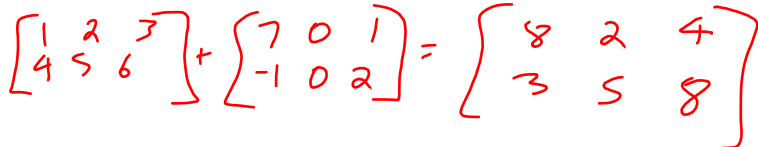
\includegraphics{img/addition-subtraction.png}

\hypertarget{scalar-multiplication}{%
\subsubsection{Scalar Multiplication}\label{scalar-multiplication}}

\begin{itemize}
\tightlist
\item
  Scalar multiplication is defined as multiplying each element of a
  matrix by a number 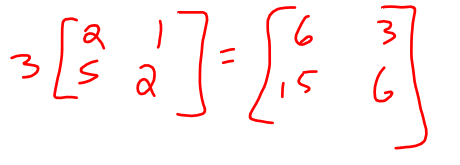
\includegraphics{img/scalar.png}
\end{itemize}

\hypertarget{matrix-multiplication}{%
\subsubsection{Matrix Multiplication}\label{matrix-multiplication}}

\begin{itemize}
\tightlist
\item
  We can \textbf{only} multiply an (m x n) by (n x p) matrix.
\item
  The resulting matrix will be (m x p)
\end{itemize}

\hypertarget{properties-of-matrix-arithmetic}{%
\subsubsection{Properties of Matrix
Arithmetic}\label{properties-of-matrix-arithmetic}}

\begin{enumerate}
\def\labelenumi{(\alph{enumi})}
\tightlist
\item
  \(A + B = B + A\) \textbf{(Commutative law for addition)}
\item
  \(A + (B + C) = (A + B) + C\) \textbf{(Associative law for addition)}
\item
  \(A(BC) = (AB)C\) \textbf{(Associative law for multiplication)}
\item
  \(A(B+C) = AB + AC\) \textbf{(Left distributive law)}
\item
  \((B+C)A = BA + CA\) \textbf{(Right distributive law)}
\item
  \(A(B-C) = AB - AC\)
\item
  \((B-C)A = BA - CA\)
\item
  a(B+C) = aB + aC
\item
  a(B-C) = aB - aC
\item
  (a+b)C = aC + bC
\item
  (a-b)C = aC - bC
\item
  a(bC) = (ab)C
\item
  a(BC) = (aB)C = B(aC)
\end{enumerate}

\hypertarget{examples}{%
\subsubsection{Examples}\label{examples}}

\begin{enumerate}
\def\labelenumi{\arabic{enumi}.}
\item
  \begin{align*}
  &\begin{bmatrix} 1 & 2 \\ 3 & 4\end{bmatrix}\begin{bmatrix} 1 & 2 \\ 3 & 4 \end{bmatrix} \\
  &= \begin{bmatrix} 1 \cdot 1 + 2 \cdot 3 & 1 \cdot 2 + 2 \cdot 4 \\ 3 \cdot 1 + 4 \cdot 3 & 3 \cdot 2 + 4 \cdot 4 \end{bmatrix} \\
  &= \begin{bmatrix} 7 & 10 \\ 15 & 22 \end{bmatrix}
  \end{align*}
\item
  \begin{align*}
  &\begin{bmatrix}2 & -3 \\ 5 & 0 \\ -2 & 4 \\ 1 & 2 \end{bmatrix}\begin{bmatrix}-1 \\ 3 \end{bmatrix} \\
  &=\begin{bmatrix} 2 \cdot (-1) + (-3) \cdot 3 \\ 5 \cdot (-1) + 0 \cdot 3 \\ -2 \cdot (-1) + 4 \cdot 3 \\ 1 \cdot (-1) + 2 \cdot 3 \end{bmatrix} \\
  &=\begin{bmatrix} -11 \\ -5 \\ 14 \\ 5 \end{bmatrix}
  \end{align*}
\item
  \begin{align*}
  &\begin{bmatrix}4 & 5 & -1 \end{bmatrix}\begin{bmatrix} 8 \\ 0 \\ 2\end{bmatrix} \\
  &= \begin{bmatrix} 4 \cdot 8 + 5 \cdot 0 + (-1) \cdot 2 \end{bmatrix} \\
  &= \begin{bmatrix} 30 \end{bmatrix}
  \end{align*}
\end{enumerate}

\hypertarget{transpose-of-a-matrix}{%
\subsection{Transpose of a Matrix}\label{transpose-of-a-matrix}}

The transpose of an (m x n) matrix is the (n x m) matrix where the rows
and columns are swapped.

If
\(B = \begin{bmatrix} 4 & 2 \\ -1 & 0 \\ 3 & 5 \end{bmatrix}, B^T = \begin{bmatrix} 4 & -1 & 3 \\ 2 & 0 & 5 \end{bmatrix}\)

\begin{align*}
B \cdot B^T &= \begin{bmatrix} 4 & 2 \\ -1 & 0 \\ 3 & 5 \end{bmatrix} \begin{bmatrix} 4 & -1 & 3 \\ 2 & 0 & 5 \end{bmatrix} \\ 
&= \begin{bmatrix} 4 \cdot 4 + 2 \cdot 2 & 4 \cdot (-1) + 2 \cdot 0 & 4 \cdot 3 + 2 \cdot 5 \\ (-1) \cdot 4 + 0 \cdot 2 & (-1) \cdot (-1) + 0 \cdot 0 & (-1) \cdot 3 + 0 \cdot 5 \\ 3 \cdot 4 + 5 \cdot 2 & 3 \cdot (-1) + 5 \cdot 0 & 3 \cdot 3 + 5 \cdot 5 \end{bmatrix} \\ 
&= \begin{bmatrix} 20 & -4 & 22 \\ -4 & 1 & -3 \\ 22 & -3 & 34\end{bmatrix}
\end{align*}

\begin{itemize}
\tightlist
\item
  The transpose of a matrix is \textbf{always} multiplicative with the
  original.
\item
  There is also a \textbf{main diagonal} that is the diagonal from the
  top left to the bottom right, but only square matrices have these.
\item
  The \textbf{trace} of a square matrix \(A\) is equal to the sum of all
  the elements on the main diagonal: \(\mathrm{tr}(A)\)
\end{itemize}

\hypertarget{transpose-matrix-properties}{%
\subsubsection{Transpose Matrix
Properties}\label{transpose-matrix-properties}}

\begin{itemize}
\tightlist
\item
  \((A^T)^T = A\)
\item
  \((A + B)^T = A^T + B^T\)
\item
  \((A - B)^T = A^T - B^T\)
\item
  \((kA)^T = kA^T\)
\item
  \((AB)^T = B^T A^T\)
\end{itemize}

\hypertarget{homework-matrix-stuff-08032023}{%
\subsection{Homework --- ``Matrix Stuff''
(08/03/2023)}\label{homework-matrix-stuff-08032023}}

\hypertarget{suppose-that-a-b-c-d-and-e-are-matrices-with-the-following-sizes}{%
\subsubsection{\texorpdfstring{Suppose that \(A, B, C, D\) and \(E\) are
matrices with the following
sizes:}{Suppose that A, B, C, D and E are matrices with the following sizes:}}\label{suppose-that-a-b-c-d-and-e-are-matrices-with-the-following-sizes}}

\begin{align*}
&A& &B& &C& &D& &E& \\
&(3 \times 2)& &(2 \times 3)& &(3 \times 3)& &(3 \times 2)& &(2 \times 3)&
\end{align*}

For each matrix operation, sort them into undefined if the operation
can't be done, or defined if it can along with the correct dimensions of
the outcome.

\begin{longtable}[]{@{}
  >{\raggedright\arraybackslash}p{(\columnwidth - 6\tabcolsep) * \real{0.1279}}
  >{\raggedright\arraybackslash}p{(\columnwidth - 6\tabcolsep) * \real{0.2907}}
  >{\raggedright\arraybackslash}p{(\columnwidth - 6\tabcolsep) * \real{0.2907}}
  >{\raggedright\arraybackslash}p{(\columnwidth - 6\tabcolsep) * \real{0.2907}}@{}}
\toprule\noalign{}
\begin{minipage}[b]{\linewidth}\raggedright
Undefined
\end{minipage} & \begin{minipage}[b]{\linewidth}\raggedright
Defined; (\(4 \times 2\))
\end{minipage} & \begin{minipage}[b]{\linewidth}\raggedright
Defined; (\(5 \times 5\))
\end{minipage} & \begin{minipage}[b]{\linewidth}\raggedright
Defined; (\(5 \times 2\))
\end{minipage} \\
\midrule\noalign{}
\endhead
\bottomrule\noalign{}
\endlastfoot
\(BA\) & \(AC + D\) & \(E(A+B)\) & \((A^T+E)D\) \\
\(AB + B\) & & & \(E(AC)\) \\
\(E^T A\) & & & \\
\(AE + B\) & & & \\
\end{longtable}

\hypertarget{consider-the-matrices}{%
\subsubsection{Consider the matrices}\label{consider-the-matrices}}

\[
A = \begin{bmatrix}3 & 0 \\ -1 & 2 \\ 1 & 1 \end{bmatrix}, B=\begin{bmatrix}4 & -1 \\ 0 & 2 \end{bmatrix}, C = \begin{bmatrix} 1 & 4 & 2 \\ 3 & 1 & 5 \end{bmatrix}, D = \begin{bmatrix} 1 & 5 & 2 \\ -1 & 0 & 1 \\ 3 & 2 & 4 \end{bmatrix}, E = \begin{bmatrix} 6 & 1 & 3 \\ -1 & 1 & 2 \\ 4 & 1 & 3 \end{bmatrix}
\]

In each part, compute the given expression (where possible).

\begin{enumerate}
\def\labelenumi{\arabic{enumi}.}
\setcounter{enumi}{1}
\item
  \(\symbf{2A^T + C}\) \begin{align*}
  2A^T + C &= 2\begin{bmatrix}3 & 0 \\ -1 & 2 \\ 1 & 1 \end{bmatrix}^T + \begin{bmatrix} 1 & 4 & 2 \\ 3 & 1 & 5 \end{bmatrix} \\ 
  &= 2\begin{bmatrix}3 & -1 & 1 \\ 0 & 2 & 1 \end{bmatrix} + \begin{bmatrix} 1 & 4 & 2 \\ 3 & 1 & 5 \end{bmatrix} \\
  &= \begin{bmatrix} 6 & -2 & 2 \\ 0 & 4 & 2 \end{bmatrix} + \begin{bmatrix} 1 & 4 & 2 \\ 3 & 1 & 5 \end{bmatrix} \\
  &= \begin{bmatrix} 7 & 2 & 4 \\ 3 & 5 & 7 \end{bmatrix}
  \end{align*}
\item
  \(\symbf{B^T + 5C^T}\) \begin{align*}
  B^T + 5C^T &= \begin{bmatrix}4 & -1 \\ 0 & 2 \end{bmatrix}^T + 5\begin{bmatrix} 1 & 4 & 2 \\ 3 & 1 & 5 \end{bmatrix}^T \\
  &= \begin{bmatrix}4 & 0 \\ -1 & 2 \end{bmatrix} + 5\begin{bmatrix} 1 & 3 \\ 4 & 1 \\ 2 & 5 \end{bmatrix} \\
  &= \begin{bmatrix}4 & 0 \\ -1 & 2 \end{bmatrix} + \begin{bmatrix} 5 & 15 \\ 20 & 5 \\ 10 & 25 \end{bmatrix} \\
  &= \text{Undefined}
  \end{align*}
\item
  \(\symbf{2E^T - 3D^T}\) \begin{align*}
  2E^T - 3D^T &= 2\begin{bmatrix} 6 & 1 & 3 \\ -1 & 1 & 2 \\ 4 & 1 & 3 \end{bmatrix}^T - 3\begin{bmatrix} 1 & 5 & 2 \\ -1 & 0 & 1 \\ 3 & 2 & 4 \end{bmatrix}^T \\
  &= 2\begin{bmatrix} 6 & -1 & 4 \\ 1 & 1 & 1 \\ 3 & 2 & 3 \end{bmatrix} - 3\begin{bmatrix} 1 & -1 & 3 \\ 5 & 0 & 2 \\ 2 & 1 & 4 \end{bmatrix} \\
  &= \begin{bmatrix} 12 & -2 & 8 \\ 2 & 2 & 2 \\ 6 & 4 & 6 \end{bmatrix} - \begin{bmatrix} 3 & -3 & 9 \\ 15 & 0 & 6 \\ 6 & 3 & 12 \end{bmatrix} \\
  &= \begin{bmatrix} 9 & -5 & -1 \\ -13 & 2 & -4 \\ 0 & 1 & -6 \end{bmatrix}
  \end{align*}
\item
  \(\symbf{\mathrm{tr}(DE)}\) \begin{align*}
  &\mathrm{tr}(DE) = \mathrm{tr}\left(\begin{bmatrix}1 & 5 & 2 \\ -1 & 0 & 1 \\ 3 & 2 & 4 \end{bmatrix}\begin{bmatrix}6 & 1 & 3 \\ -1 & 1 & 2 \\ 4 & 1 & 3 \end{bmatrix}\right) \\
  &= \mathrm{tr}\left(\begin{bmatrix}1 \cdot 6 + 5 \cdot (-1) + 2 \cdot 4 & 1 \cdot 1 + 5 \cdot 1 + 2 \cdot 1 & 1 \cdot 3 + 5 \cdot 2 + 2 \cdot 3 \\ (-1) \cdot 6 + 0 \cdot (-1) + 1 \cdot 4 & (-1) \cdot 1 + 0 \cdot 1 + 1 \cdot 1 & (-1) \cdot 3 + 0 \cdot 2 + 1 \cdot 3 \\ 3 \cdot 6 + 2 \cdot (-1) + 4 \cdot 4 & 3 \cdot 1 + 2 \cdot 1 + 4 \cdot 1 & 3 \cdot 3 + 2 \cdot 2 + 4 \cdot 3 \end{bmatrix}\right) \\
  &= \mathrm{tr}\left(\begin{bmatrix} 9 & 8 & 19 \\ -2 & 0 & 0 \\ 32 & 9 & 25 \end{bmatrix}\right) \\
  &= 34
  \end{align*}
\end{enumerate}

\hypertarget{intro-to-systems}{%
\section{Intro to Systems}\label{intro-to-systems}}

What are we looking for?

Lines: How many possible solutions?

\begin{itemize}
\tightlist
\item
  Infinite solutions
\item
  One solution
\item
  No solutions
\end{itemize}

Planes: How many possible solutions?

\begin{itemize}
\tightlist
\item
  Infinite solutions
\item
  No solutions
\end{itemize}

What does linear actually mean?

\begin{itemize}
\tightlist
\item
  The word linear \emph{really} means that you've got equations with
  variables and \textbf{all} of the variables are degree one.
\item
  This means that there is no limit to the number of dimensions in a
  linear system.
\end{itemize}

\begin{center}
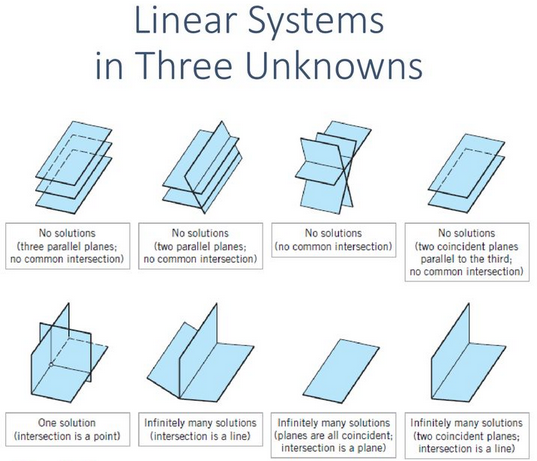
\includegraphics[width=0.8\textwidth,height=\textheight]{img/linearsystems.png}
\end{center}

\hypertarget{review-solve-the-following-systems}{%
\subsection{Review: Solve the following
systems}\label{review-solve-the-following-systems}}

\begin{enumerate}
\def\labelenumi{\arabic{enumi}.}
\item
  \systeme{2x+y=10, 3x-y=5}

  \begin{align*}
  5x &= 15 \\
  x &= 3 \\
  2(3)+y &= 10 \\
  6 + y &= 10 \\
  y &= 4
  \end{align*}
\item
  \systeme{2x+y=10, 6x+3y=10}

  \begin{align*}
  y &= 10-2x \\
  6x + 3(10-2x) &= 10 \\
  6x + 30 - 6x &= 10 \\
  30 &= 10 \therefore \text { no solution}
  \end{align*}
\item
  \systeme{5x-2y=4, 15x-6y=12}

  \begin{align*}
  0 &= 0 \\
  12 &= 12 \therefore \text{ infinite solutions}
  \end{align*}
\end{enumerate}

\begin{multicols}{2}
  \hypertarget{review-solve-the-following-systems}{%
  \subsubsection{Consistent}\label{consistent}}

  \begin{itemize}
    \tightlist
    \item A system of equations is \textbf{consistent} if it has at least one solution.
  \end{itemize}

\columnbreak

  \hypertarget{review-solve-the-following-systems}{%
  \subsubsection{Inconsistent}\label{inconsistent}}

  \begin{itemize}
    \tightlist
    \item A system of equations is \textbf{inconsistent} if it has no solutions.
  \end{itemize}

\end{multicols}

\newpage{}

\hypertarget{the-augmented-matrix}{%
\subsection{The Augmented Matrix}\label{the-augmented-matrix}}

\Large\systeme{x-y+2z=5,2x-2y+4z=10,3x-3y+6z=15}
\(\longrightarrow \left[\begin{array}{ccc|c}1 & -1 & 2 & 5 \\ 2 & -2 & 4 & 10 \\ 3 & -3 & 6 & 15 \end{array}\right]\)
\normalsize

\hypertarget{elementary-row-operations}{%
\subsection{Elementary Row Operations}\label{elementary-row-operations}}

\begin{enumerate}
\def\labelenumi{\arabic{enumi}.}
\tightlist
\item
  Interchange 2 rows
\item
  Multiply a row by a non-zero constant
\item
  Add/substract a multiple of one row to/from another row
\end{enumerate}

Doing these things changes the matrix, but it's the same system!

\hypertarget{example-1-again}{%
\subsubsection{Example 1\ldots{} again}\label{example-1-again}}

\systeme{2x+y=10, 3x-y=5}

\begin{align*}
\Large
\left[\begin{array}{cc|c}2 & 1 & 10 \\ 3 & -1 & 5 \end{array} \right]&\rowops{\frac{1}{2}R_1,}\left[\begin{array}{cc|c}1 & \frac{1}{2} & 5 \\ 3 & -1 & 5 \end{array} \right] \rowops{,R_2-3R_1}\left[\begin{array}{cc|c}1 & \frac{1}{2} & 5 \\ 0 & -\frac{5}{2} & -10 \end{array}\right] \\
&\rowops{,-\frac{2}{5}R_2} \left[\begin{array}{cc|c}1 & \frac{1}{2} & 5 \\ 0 & 1 & 4 \end{array}\right]\rowops{R1-\frac{1}{2}R_2,}\left[\begin{array}{cc|c}1 & 0 & 3 \\ 0 & 1 & 4 \end{array}\right]
\end{align*}

And so\ldots{} \(x=3\) and \(y=4\)!

\hypertarget{connection-to-matrices}{%
\subsection{Connection to Matrices}\label{connection-to-matrices}}

If we can make a system's matrix look like

\(\left[\begin{array}{ccc|c}1 & 0 & 0 & c_1 \\ 0 & 1 & 0 & c_2 \\ 0 & 0 & 1 & c_3 \end{array}\right]\),

then the solution to the system will be the ordered triple
\((c_1, c_2, c_3)\).

\hypertarget{example-2-again}{%
\subsubsection{Example 2: again}\label{example-2-again}}

\systeme{2x+y=10, 6x+3y=10}

\begin{align*}
\left[\begin{array}{cc|c}2 & 1 & 10 \\ 6 & 3 & 10 \end{array}\right] \rowops{\frac{1}{2}R1,} \left[\begin{array}{cc|c}1 & \frac{1}{2} & 5 \\ 6 & 3 & 10 \end{array}\right] \rowops{,R2-6R1,} \left[\begin{array}{cc|c}1 & \frac{1}{2} & 5 \\ 0 & 0 & -20 \end{array}\right]
\end{align*}

This is inconsistent, so there is no solution.

\hypertarget{example-3-again}{%
\subsubsection{Example 3: again}\label{example-3-again}}

\systeme{5x-2y=4, 15x-6y=12}

\begin{align*}
\left[\begin{array}{cc|c}5 & -2 & 4 \\ 15 & -6 & 12\end{array}\right]\rowops{\frac{1}{5}R1,}\left[\begin{array}{cc|c}1 & -\frac{2}{5} & \frac{4}{5} \\ 15 & -6 & 12 \end{array}\right]\rowops{,R2-15R1}\left[\begin{array}{cc|c}1 & -\frac{2}{5} & \frac{4}{5} \\ 0 & 0 & 0 \end{array}\right]
\end{align*}

Since \(0 = 0\), there are infinitely many solutions.

\hypertarget{example-4-solve-the-following-system}{%
\subsubsection{Example 4: Solve the following
system}\label{example-4-solve-the-following-system}}

\systeme{x_1-2x_2 + x_3 = 0, 2x_2-8x_3=8, -4x_1+5x_2+9x_3=-9}

\begin{align*}
&\left[\begin{array}{ccc|c}
1 & -2 & 1 & 0 \\ 0 & 2 & -8 & 8 \\ -4 & 5 & 9 & -9
\end{array}\right]\rowops{R3+4R1,}\left[\begin{array}{ccc|c}1 & -2 & 1 & 0 \\ 0 & 2 & -8 & 8 \\ 0 & -3 & 13 & -9 \end{array}\right]\rowops{,R3+\frac{3}{2}R2,}\left[\begin{array}{ccc|c}1 & -2 & 1 & 0 \\ 0 & 2 & -8 & 8 \\ 0 & 0 & -1 & 3 \end{array}\right] \\
&\rowops{,\frac{1}{2}R_2,}
\left[\begin{array}{ccc|c}
1 & -2 & 1 & 0 \\ 0 & 1 & -4 & 4 \\ 0 & -3 & 13 & -9 
\end{array}\right] \rowops{R_1+2R_2,,R_3+3R_2}\left[\begin{array}{ccc|c}
1 & 0 & -7 & 8 \\ 0 & 1 & -4 & 4 \\ 0 & 0 & 1 & 3
\end{array}\right]\rowops{R1+7R_3,R_2+4R_3,}\left[\begin{array}{ccc|c}
1 & 0 & 0 & 29 \\ 0 & 1 & 0 & 16 \\ 0 & 0 & 1 & 3
\end{array}\right]
\end{align*}

Therefore the solution to \((x_1, x_2, x_3)\) is \((29, 16, 3)\).

\hypertarget{elementary-row-operations-ref-homework-problem-08082023}{%
\subsubsection{Elementary Row Operations \& REF Homework Problem
(08/08/2023)}\label{elementary-row-operations-ref-homework-problem-08082023}}

\systeme{x + y + 2z = 8, -x - 2y + 3z = 1, 3x - 7y + 4z = 10}

\begin{align*}
&\left[\begin{array}{ccc|c}
1 & 1 & 2 & 8 \\
-1 & -2 & 3 & 1 \\
3 & -7 & 4 & 10
\end{array}\right]\rowops{,R_2+R_1,R_3-3R_1}
\left[\begin{array}{ccc|c}
1 & 1 & 2 & 8 \\
0 & -1 & 5 & 9 \\
0 & -10 & -2 & -14
\end{array}\right]\rowops{,-R_2, -R_3}\left[\begin{array}{ccc|c}
1 & 1 & 2 & 8 \\
0 & 1 & -5 & -9 \\
0 & 10 & 2 & 14
\end{array}\right] \\
&\rowops{R_1-R_2,,R_3-10R_2}\left[\begin{array}{ccc|c}
1 & 0 & 7 & 17 \\
0 & 1 & -5 & -9 \\
0 & 0 & 52 & 104
\end{array}\right]\rowops{,,\frac{1}{52}R_3}\left[\begin{array}{ccc|c}
1 & 0 & 7 & 17 \\
0 & 1 & -5 & -9 \\
0 & 0 & 1 & 2
\end{array}\right]\rowops{R_1-7R_3,R_2+5R_3,}\left[\begin{array}{ccc|c}
1 & 0 & 0 & 3 \\
0 & 1 & 0 & 1 \\
0 & 0 & 1 & 2
\end{array}\right]
\end{align*}

Therefore, the solution to \((x, y, z)\) is \((3, 1, 2)\).

\hypertarget{gaussian-elimination}{%
\subsection{Gaussian Elimination}\label{gaussian-elimination}}

\ul{Vocabulary}: A matrix is in \ul{Row Echelon Form (REF)} if:

\begin{enumerate}
\def\labelenumi{(\alph{enumi})}
\tightlist
\item
  Any rows of all zeroes are placed at the bottom of the matrix
\item
  All other rows have a \ul{leading 1} (``pivot'')
\item
  As we move down the matrix, each leading 1 is further to the right
  than the 1 above it
\end{enumerate}

A matrix is in \ul{Row Reduced Echelon Form} if the three above
conditions are met in adition to:

\begin{enumerate}
\def\labelenumi{(\alph{enumi})}
\setcounter{enumi}{3}
\tightlist
\item
  Each column with a leading 1 has all other entries in the column as a
  0. (``pivot column'')
\end{enumerate}

\newpage{}

\hypertarget{examples-1}{%
\subsubsection{Examples}\label{examples-1}}

\begin{multicols}{2}
$\begin{bmatrix}1 & 0 & 0 & 0 & 8\\ 0 & 1 & 0 & 6 & -3 \\ 0 & 0 & 1 & 7 & 10\\ 0 & 0 & 0 & 0 & 0 \end{bmatrix}$

$\begin{bmatrix}1 & 1 & 1 & 0 \\ 0 & 1 & 1 & 0 \\ 0 & 0 & 0 & 1 \end{bmatrix}$

$\begin{bmatrix}1 & 2 & -3 & 4 \\ 0 & 0 & 0 & 0 \\ 0 & 1 & 2 & -4\end{bmatrix}$
\columnbreak

REF? \checkmark \\
RREF? \checkmark \\

\vspace{1cm}

REF? \checkmark \\
RREF? \times \\

\vspace{1cm}

REF? \times \\
RREF? \times

\end{multicols}

\hypertarget{gaussian-elimination-with-back-substitution}{%
\subsection{\texorpdfstring{Gaussian Elimination With
\textbf{Back-Substitution}}{Gaussian Elimination With Back-Substitution}}\label{gaussian-elimination-with-back-substitution}}

\hypertarget{goal}{%
\subsubsection{Goal:}\label{goal}}

To get the augmented matrix in REF

Solve:
\systeme{x_1 - 2x_2 + 3x_3 = 9, -x_1 + 3x_2 = -4, 2x_1 - 5x_2 + 5x_3 = 17}
\begin{align*}
&\left[\begin{array}{ccc|c}1 & -2 & 3 & 9 \\ -1 & 3 & 0 & -4 \\ 2 & -5 & 5 & 17 \end{array}\right]\rowops{,R_2+R_1,R_3-2R_1}\left[\begin{array}{ccc|c}1 & -2 & 3 & 9 \\ 0 & 1 & 3 & 5 \\ 0 & -1 & -1 & -1 \end{array}\right]\rowops{R_1+2R_2,,R_3+R_2}\left[\begin{array}{ccc|c}1 & 0 & 9 & 19 \\ 0 & 1 & 3 & 5 \\ 0 & 0 & 2 & 4 \end{array}\right] \\
&\rowops{,,\frac{1}{2}R_3}\left[\begin{array}{ccc|c}1 & 0 & 9 & 19 \\ 0 & 1 & 3 & 5 \\ 0 & 0 & 1 & 2\end{array}\right]
\end{align*} \begin{align*}
x + 9z &= 19 \\
y + 3z &= 5 \\
z &= 2 \\
\therefore \ z &= 2, y = 5-3z, x = 19-9z \\
z &= 2, y = 5-3(2), x = 19-9(2) \\
z &= 2, y = -1, x = 1
\end{align*} Therefore, the solution \((x_1, x_2, x_3)\) is
\((1, -1, 2)\).

\hypertarget{gaussian-elimination-homework-problem-08092023}{%
\subsubsection{Gaussian Elimination Homework Problem
(08/09/2023)}\label{gaussian-elimination-homework-problem-08092023}}

\systeme{y+z-2w=-3, x+2y-z=2,2x+4y+z-3w=-2,x-4y-7z-w=-19}

\begin{align*}
&\left[\begin{array}{cccc|c}-2 & 0 & 1 & 1 & -3 \\ 0 & 1 & 2 & -1 & 2 \\ -3 & 2 & 4 & 1 & -2 \\ -1 & 1 & -4 & -7 & -19\end{array}\right]\rowops{R_4,,,R_1}\left[\begin{array}{cccc|c} -1 & 1 & -4 & -7 & -19 \\ 0 & 1 & 2 & -1 & 2 \\ -3 & 2 & 4 & 1 & -2 \\ -2 & 0 & 1 & 1 & -3\end{array}\right]\rowops{-R_1,,,} \\
&\left[\begin{array}{cccc|c} 1 & -1 & 4 & 7 & 19 \\  0 & 1 & 2 & -1 & 2 \\ -3 & 2 & 4 & 1 & -2 \\ -2 & 0 & 1 & 1 & -3\end{array}\right]\rowops{,,R_3+3R_1,R_4+2R_1}\left[\begin{array}{cccc|c} 1 & -1 & 4 & 7 & 19 \\ 0 & 1 & 2 & -1 & 2 \\ 0 & -1 & 16 & 22 & 55 \\ 0 & -2 & 9 & 15 & 35\end{array}\right]\rowops{R_1+R_2,,R_3+R_2,R_4+2R_2} \\
&\left[\begin{array}{cccc|c}1 & 0 & 6 & 6 & 21 \\ 0 & 1 & 2 & -1 & 2 \\ 0 & 0 & 18 & 21 & 57 \\ 0 & 0 & 13 & 13 & 39 \end{array}\right]\rowops{,,\frac{1}{18}R_3,}\left[\begin{array}{cccc|c}1 & 0 & 6 & 6 & 21 \\ 0 & 1 & 2 & -1 & 2 \\ 0 & 0 & 1 & \frac{7}{6} & \frac{19}{6} \\ 0 & 0 & 13 & 13 & 39 \end{array}\right]\rowops{R_1-6R_3,R_2-2R_3,,R_4-13R_3} \\
&\left[\begin{array}{cccc|c}1 & 0 & 0 & -1 & 2 \\ 0 & 1 & 0 & -\frac{10}{3} & -\frac{13}{3} \\ 0 & 0 & 1 & \frac{7}{6} & \frac{19}{6} \\ 0 & 0 & 0 & -\frac{13}{6} & -\frac{13}{6} \end{array}\right]\rowops{,,,\frac{-6}{13}R_4}\left[\begin{array}{cccc|c}1 & 0 & 0 & -1 & 2 \\ 0 & 1 & 0 & -\frac{10}{3} & -\frac{13}{3} \\ 0 & 0 & 1 & \frac{7}{6} & \frac{19}{6} \\ 0 & 0 & 0 & 1 & 1 \end{array}\right]\rowops{R_1+R_4,R_2+\frac{10}{3}R_4,R_3-\frac{7}{6}R_4,} \\
&\left[\begin{array}{cccc|c}1 & 0 & 0 & 0 & 3 \\ 0 & 1 & 0 & 0 & -1 \\ 0 & 0 & 1 & 0 & 2 \\ 0 & 0 & 0 & 1 & 1 \end{array}\right] \Longrightarrow \systeme*{w=3, x=-1, y=2, z=1}
\end{align*}

\newpage{}

\hypertarget{gauss-jordan-elimination}{%
\subsection{Gauss-Jordan Elimination}\label{gauss-jordan-elimination}}

\hypertarget{goal-1}{%
\subsubsection{Goal:}\label{goal-1}}

To get the matrix into RREF

Solve: \systeme{x_1-3x_3=-2, 3x_1+x_2-2x_3=5, 2x_1+2x_2+x_3=4}

\begin{align*}
&\left[\begin{array}{ccc|c}1 & 0 & -3 & -2 \\ 3 & 1 & -2 & 5 \\ 2 & 2 & 1 & 4\end{array}\right]\rowops{,R_2-3R_1,R_3-2R_1}\left[\begin{array}{ccc|c}1 & 0 & -3 & -2 \\ 0 & 1 & 7 & 11 \\ 0 & 2 & 7 & 8\end{array}\right]\rowops{,,R_3-2R_2}\left[\begin{array}{ccc|c}1 & 0 & -3 & -2 \\ 0 & 1 & 7 & 11 \\ 0 & 0 & -7 & -14\end{array}\right]\\
&\rowops{,,\frac{-1}{7}R_3}\left[\begin{array}{ccc|c}1 & 0 & -3 & -2 \\ 0 & 1 & 7 & 11 \\ 0 & 0 & 1 & 2\end{array}\right]\rowops{R_1+3R_3,R_2-7R_3,}\left[\begin{array}{ccc|c}1 & 0 & 0 & 4 \\ 0 & 1 & 0 & -3 \\ 0 & 0 & 1 & 2\end{array}\right] \Longrightarrow \systeme*{x_1=4, x_2=-3, x_3=2}
\end{align*}

\hypertarget{matrix-properties-equations-and-inverses}{%
\subsection{Matrix Properties, Equations, and
Inverses}\label{matrix-properties-equations-and-inverses}}

\hypertarget{with-real-numbers}{%
\subsubsection{With Real Numbers}\label{with-real-numbers}}

\begin{itemize}
\tightlist
\item
  If \(ab = bc\), then \(a = c\), if \(b \ne 0\)
\item
  If \(ab = 0\), then \(a = 0\) or \(b = 0\), or both
\end{itemize}

\hypertarget{with-matrices}{%
\subsubsection{With Matrices}\label{with-matrices}}

\begin{itemize}
\tightlist
\item
  If \(AB = AC\), then \(B = C\), if \(A\) is invertible
\item
  If \(AB = [0]\), then \(A = [0]\) or \(B = [0]\), or both
\end{itemize}

\hypertarget{multiply}{%
\paragraph{Multiply:}\label{multiply}}

\begin{align*}
&\begin{bmatrix} 2 & 3 \\ 3 & 5 \end{bmatrix}
\begin{bmatrix} 5 & -3 \\ -3 & 2 \end{bmatrix} \\
&= \begin{bmatrix} 2(5)+3(-3) & 2(-3)+3(2) \\ 3(5)+5(-3) & 3(-3)+5(2) \end{bmatrix} \\
&= \begin{bmatrix} 1 & 0 \\ 0 & 1 \end{bmatrix}
\end{align*}

\hypertarget{matrix-inverses}{%
\subsubsection{Matrix Inverses}\label{matrix-inverses}}

\begin{itemize}
\item
  If a matrix has an inverse, it is said to be invertible or
  non-singular.
\item
  If a matrix does not have an inverse, it is said to be singular.
\item
  Every square matrix has a ``special number'' associated with it called
  the \textbf{determinant}.
\item
  For the \(2 \times 2\) matrix
  \(A = \begin{bmatrix}a & b \\ c & d \end{bmatrix}\), the determinant
  is \(ad-bc\)
\item
  \(A^{-1} = \frac{1}{\det{A}}\begin{bmatrix}d & -b \\ -c & a \end{bmatrix}\)
\item
  When \(\det{A} = 0\), the matrix is singular and has no inverse (since
  you cannot divide by zero)
\end{itemize}

Find the inverse of \(A = \begin{bmatrix}4 & 3 \\ 1 & 2 \end{bmatrix}\)

\begin{align*}
&\begin{bmatrix}4 & 3 \\ 1 & 2 \end{bmatrix}^{-1} &= \frac{1}{\det{A}}\begin{bmatrix}2 & -3 \\ -1 & 4 \end{bmatrix} \\
&= \frac{1}{(4)(2)-(3)(1)}\begin{bmatrix}2 & -3 \\ -1 & 4 \end{bmatrix} \\
&= \frac{1}{5}\begin{bmatrix}2 & -3 \\ -1 & 4 \end{bmatrix} \\
&= \begin{bmatrix}\frac{2}{5} & -\frac{3}{5} \\ -\frac{1}{5} & \frac{4}{5} \end{bmatrix}
\end{align*}

\hypertarget{chapter-2-determinants}{%
\section{Chapter 2: Determinants}\label{chapter-2-determinants}}

\hypertarget{prior-knowledge}{%
\subsection{Prior Knowledge:}\label{prior-knowledge}}

\(\begin{bmatrix}10 & -4 \\ -3 & -5 \end{bmatrix}=-50-=-62\)
\begin{align*}
&\begin{bmatrix}2 & 4 & 3 \\ -1 & 2 & 3 \\ 3 & 0 & -2 \end{bmatrix} \\
&= ((2\cdot2\cdot-2) + (4\cdot3\cdot3)+(3\cdot-1\cdot0))-((3\cdot2\cdot3)+(0\cdot3\cdot2)+(-2\cdot-1\cdot4)) \\
&= (-8+36+0)-(18+0+8) \\
&= 28-26 \\
&= 2
\end{align*}

\hypertarget{minors-cofactors}{%
\subsection{Minors \& Cofactors}\label{minors-cofactors}}

Given a square matrix A, the \ul{minor} of matrix element \(a_{ij}\),
(\(M_{ij}\)) is the determinant of the matrix formed by removing the
\(i^{\text{th}}\) row and \(j^{\text{th}}\) column from matrix A.

The \ul{cofactor} of matrix element
\(a_{ij}, C_{ij}=(-1)^{i+j}\cdot M_{ij}\)

\hypertarget{example}{%
\subsubsection{Example}\label{example}}

Let \(\det\begin{bmatrix}2&4&3 \\ -1&2&3 \\ 3&0&-2\end{bmatrix}\). What
is the cofactor of element (1, 1)?

Cofactor checkerboard:\\
\(\begin{bmatrix}+ & - & + \\ - & + & - \\ + & - & +\end{bmatrix}\)

\(M_{11} = \begin{vmatrix}2 & 3 \\ 0 & -2\end{vmatrix} = -4\)\\
\(C_{11} = 1 \cdot -4 = -4\)

Find the minor and cofactor of: \textbackslash{} a) \(a_{21} = -1\)
\begin{align*}
M_{21} = \begin{vmatrix}4 & 3 \\ 0 & -2 \end{vmatrix} = -8 \\
C_{21} = 8
\end{align*} b) \(a_{33} = -2\) \begin{align*}
M_{33} = \begin{vmatrix}2 & 4 \\ -1 & 2 \end{vmatrix} = 8 \\
C_{33} = 8
\end{align*}

\hypertarget{cofactor-expansion}{%
\subsection{Cofactor Expansion}\label{cofactor-expansion}}

\begin{enumerate}
\def\labelenumi{\arabic{enumi})}
\tightlist
\item
  Pick a row or column
\item
  Multiply every entry in that row or column by it's corresponding
  cofactor
\item
  Add those together. That's it
\end{enumerate}

\(A = \begin{bmatrix} 6 & 7 & -1 \\ 0 & 4 & 1 \\ 2 & 5 & -3\end{bmatrix}\)
\begin{align*}
\det(A) &= 6\left(\begin{vmatrix}4 & 1 \\ 5 & -3\end{vmatrix}\right) + 7\left(-\begin{vmatrix}0 & 1 \\ 2 & -3\end{vmatrix}\right) + -1\left(\begin{vmatrix}0 & 4 \\ 2 & 5 \end{vmatrix}\right) \\
&=6(-17) + 7(2) + (-1(-8)) \\
&= -102+14+8 \\
&=-80
\end{align*}

\hypertarget{example-1}{%
\subsubsection{Example}\label{example-1}}

\(A = \begin{bmatrix} 6 & 4 & 2 \\ 5 & -6 & 1 \\ 0 & 3 & 0\end{bmatrix}\)
\begin{align*}
& 6\begin{vmatrix}-6 & 1 \\ 3 & 0\end{vmatrix}+4\left(-\begin{vmatrix}5&1 \\ 0 & 0\end{vmatrix}\right)+2\begin{vmatrix}5 & -6 \\ 0 & 3\end{vmatrix} \\
&= 6(-3) + 0 + 2(15) \\
&= -18 + 30 \\
&= 12
\end{align*}

\hypertarget{does-the-method-generalize-to-2x2-matrices}{%
\subsubsection{Does the method generalize to 2x2
matrices?}\label{does-the-method-generalize-to-2x2-matrices}}

\begin{align*}
&\begin{vmatrix}3 & 5 \\ 7 & 2\end{vmatrix} \\
&=3|2|-5|7| \\
&=6-35 \\
&=-29
\end{align*}

The determinant of a 1x1 matrix is\ldots{} \textbf{itself!}

\hypertarget{find-the-determinant-of-a-4x4}{%
\subsubsection{Find the determinant of a
4x4}\label{find-the-determinant-of-a-4x4}}

\(A=\begin{bmatrix}-3 & 2 & 0 & 8 \\ 2 & 1 & 0 & -4 \\ 5 & -2 & 1 & 5 \\ 2 & 3 & 0 & 6\end{bmatrix}\)

\begin{align*}
&= 0 + 0 + \begin{vmatrix}-3 & 2 & 8 \\ 2 & 1 & -4 \\ 2 & 3 & 6\end{vmatrix}+0 \\
&= -2\begin{vmatrix}2 & 8 \\ 3 & 6 \end{vmatrix} + \begin{vmatrix}-3 & 8 \\ 2 & 6 \end{vmatrix}-\left(-4\begin{vmatrix}-3 & 2 \\ 2 & 3\end{vmatrix}\right) \\
&= 24 -34 -52 \\
&= -62
\end{align*}

\hypertarget{theorem}{%
\subsection{Theorem}\label{theorem}}

If \(A\) is an \(n \times n\) matrix, then regardless of which row or
column of \(A\) is chosen, the number obtained by multiplying the
elements in that row or column by their corresponding cofactors is
\ul{\textbf{always the same}} and is called the \ul{determinant} of
\(A\).

\hypertarget{example-2}{%
\subsubsection{Example}\label{example-2}}

Find the determinant of
\(A=\begin{bmatrix}1 & 0 & 0 & -1 \\ 3 & 1 & 2 & 2 \\ 1 & 0 & -2 & 1 \\ 2 & 0 & 0 & 1\end{bmatrix}\)
\begin{align*}
&1\cdot\begin{vmatrix}1 & 0 & -1 \\ 1 & -2 & 1 \\ 2 & 0 & 1 \end{vmatrix} \\
&=\left(-2\begin{vmatrix}1 & -1 \\ 2 & 1\end{vmatrix}\right) \\
&= -6
\end{align*}

\hypertarget{triangular-matrices}{%
\subsection{Triangular Matrices}\label{triangular-matrices}}

Find the determinant of
\(A = \begin{bmatrix}1 & 1 & 1 & 1 \\ 0 & 2 & 2 & 2 \\ 0 & 0 & 3 & 3 \\ 0 & 0 & 0 & 4\end{bmatrix}\)
\begin{align*}
&\begin{vmatrix}2 & 2 & 2 \\ 0 & 3 & 3 \\ 0 & 0 & 4\end{vmatrix} \\
&= 2\begin{vmatrix}3 & 3 \\ 0 & 4\end{vmatrix} \\
&= 2(3\cdot4) \\
&= 2\cdot12 \\
&=24
\end{align*}

If \(A\) is an \(n \times n\) triangular matrix, then \(\det(A)\) is
equal to the product of the elements along the main diagonal.

\hypertarget{an-important-definition}{%
\subsection{An Important Definition}\label{an-important-definition}}

\ul{Elementary Matrix} a matrix that can be obtanied from the
\(n \times n\) identity matrix by performing a single row operation.
\textbackslash{}

Are the following matrices elementary? 1)
\(\begin{bmatrix}1 & 0 \\ -5 & 1\end{bmatrix}+(R_3+5R_1)\) yes 2)
\(\begin{bmatrix}-5 & 1 \\ 1 & 0\end{bmatrix}+(R_1+5R_2)...\) no

\hypertarget{a-pair-of-theorems}{%
\subsection{A Pair of Theorems}\label{a-pair-of-theorems}}

\hypertarget{theorem-if-a-square-matrix-a-has-a-row-of-column-of-zeros-then-deta-0}{%
\subsubsection{\texorpdfstring{Theorem: If a square matrix \(A\) has a
row of column of zeros, then
\(\det(A) = 0\)}{Theorem: If a square matrix A has a row of column of zeros, then \textbackslash det(A) = 0}}\label{theorem-if-a-square-matrix-a-has-a-row-of-column-of-zeros-then-deta-0}}

\hypertarget{theorem-if-a-is-a-square-matrix-then-deta-detat}{%
\subsubsection{\texorpdfstring{Theorem: If \(A\) is a square matrix,
then
\(\det(A) = \det(A^T)\)}{Theorem: If A is a square matrix, then \textbackslash det(A) = \textbackslash det(A\^{}T)}}\label{theorem-if-a-is-a-square-matrix-then-deta-detat}}

\newpage{}

\hypertarget{unit-1-2-homework-problems}{%
\subsection{Unit 1 \& 2 Homework
Problems}\label{unit-1-2-homework-problems}}

\hypertarget{gaussian-elimination-08112023}{%
\subsubsection{``Gaussian Elimination''
(08/11/2023)}\label{gaussian-elimination-08112023}}

\hypertarget{solve-this-system-using-gaussian-elimination}{%
\paragraph{Solve this system using Gaussian
Elimination}\label{solve-this-system-using-gaussian-elimination}}

\systeme{x_1 + x_2 + 2x_3 = 8, -x_1-2x_2+3x_3 = 1, 3x_1 - 7x_2 +4x_3=10}

\begin{equation*}
\begin{aligned}
&\Rightarrow \left[\begin{array}{ccc|c}1 & 1 & 2 & 8 \\ -1 & -2 & 3 & 1 \\ 3 & -7 & 4 & 10\end{array}\right] \rowops{,R_2+R_1,R_3-3R_1}\left[\begin{array}{ccc|c}1 & 1 & 2 & 8 \\ 0 & -1 & 5 & 9 \\ 0 & -10 & -2 & -14\end{array}\right] \rowops{,-R_2,} \left[\begin{array}{ccc|c}1 & 1 & 2 & 8 \\ 0 & 1 & -5 & -9 \\ 0 & -10 & -2 & -14\end{array}\right] \\
&\rowops{,,R_3+10R_2} \left[\begin{array}{ccc|c}1 & 1 & 2 & 8 \\ 0 & 1 & -5 & -9 \\ 0 & 0 & -52 & -104\end{array}\right]\rowops{,,-\frac{1}{52}R_3}\left[\begin{array}{ccc|c}1 & 1 & 2 & 8 \\ 0 & 1 & -5 & -9 \\ 0 & 0 & 1 & 2\end{array}\right]
\end{aligned}
\end{equation*} \(\therefore\)
\systeme{x_1+x_2+2x_3=8, x_2-5x_3=-9, x_3=2} \(\Rightarrow\)
\systeme*{x_1=3, x_2=1, x_3=2}

\hypertarget{solve-this-system-using-gaussian-elimination-1}{%
\paragraph{Solve this system using Gaussian
Elimination}\label{solve-this-system-using-gaussian-elimination-1}}

\systeme{x_1-2x_2+3x_3=0,-2x_1-3x_2-4x_3=0,2x_1-4x_2+4x_3=0}

\begin{equation*}
\begin{aligned}
\Rightarrow \left[\begin{array}{ccc|c}1 & -2 & 3 & 0 \\ -2 & -3 & -4 & 0 \\ 2 & -4 & 4 & 0\end{array}\right] \rowops{,R_2+2R_1,R_3-2R_1}\left[\begin{array}{ccc|c}1 & -2 & 3 & 0 \\ 0 & -7 & 2 & 0 \\ 0 & 0 & -2 & 0\end{array}\right] \rowops{,-\frac{1}{7}R_2,-\frac{1}{2}R_3}\left[\begin{array}{ccc|c}1 & -2 & 3 & 0 \\ 0 & 1 & \frac{2}{7} & 0 \\ 0 & 0 & 1 & 0\end{array}\right]
\end{aligned}
\end{equation*} \(\therefore\)
\systeme*{x_1-2x_2+3x_3=0, x_2+\frac{2}{7}x_3=0, x_3=0}
\(\Rightarrow 1 \ne 0 \therefore \text{ no solution}\)

\newpage{}

\hypertarget{inverses-and-determinants-0814}{%
\subsubsection{``Inverses and Determinants''
(08/14)}\label{inverses-and-determinants-0814}}

\hypertarget{find-the-determinants-of-the-following}{%
\paragraph{Find the determinants of the
following:}\label{find-the-determinants-of-the-following}}

\begin{enumerate}
\def\labelenumi{\arabic{enumi})}
\tightlist
\item
  \(\begin{bmatrix}2 & -3 \\ 4 & 4 \end{bmatrix}\)
\end{enumerate}

\(\begin{vmatrix}2 & -3 \\ 4 & 4 \end{vmatrix} = 2(4)-(-3)(4) = 8+12 = 20\)

\begin{enumerate}
\def\labelenumi{\arabic{enumi})}
\setcounter{enumi}{1}
\tightlist
\item
  \(\begin{bmatrix}2 & 0 \\ 0 & 3 \end{bmatrix}\)
\end{enumerate}

\(\begin{vmatrix}2 & 0 \\ 0 & 3 \end{vmatrix} = 2(3)-0(0) = 6\)

\begin{enumerate}
\def\labelenumi{\arabic{enumi})}
\setcounter{enumi}{2}
\tightlist
\item
  \(\begin{bmatrix}\cos\theta & \sin\theta \\ -\sin\theta & \cos\theta \end{bmatrix}\)
\end{enumerate}

\(\begin{vmatrix}\cos\theta & \sin\theta \\ -\sin\theta & \cos\theta \end{vmatrix} = \cos^2\theta + \sin^2\theta = 1\)

\hypertarget{find-the-inverses-of-those-matrices}{%
\paragraph{Find the INVERSES of those
matrices:}\label{find-the-inverses-of-those-matrices}}

\begin{enumerate}
\def\labelenumi{\arabic{enumi})}
\tightlist
\item
  \(\begin{bmatrix}2 & -3 \\ 4 & 4 \end{bmatrix}\)
\end{enumerate}

\(\begin{bmatrix}2 & -3 \\ 4 & 4 \end{bmatrix}^{-1} = \frac{1}{20}\begin{bmatrix}4 & 3 \\ -4 & 2 \end{bmatrix}=\begin{bmatrix}\frac{1}{5} & \frac{3}{20} \\ -\frac{1}{5} & \frac{1}{10}\end{bmatrix}\)

\begin{enumerate}
\def\labelenumi{\arabic{enumi})}
\setcounter{enumi}{1}
\tightlist
\item
  \(\begin{bmatrix}2 & 0 \\ 0 & 3 \end{bmatrix}\)
\end{enumerate}

\(\begin{bmatrix}2 & 0 \\ 0 & 3 \end{bmatrix}^{-1} = \frac{1}{6}\begin{bmatrix}3 & 0 \\ 0 & 2 \end{bmatrix}=\begin{bmatrix}\frac{1}{2} & 0 \\ 0 & \frac{1}{3}\end{bmatrix}\)

\begin{enumerate}
\def\labelenumi{\arabic{enumi})}
\setcounter{enumi}{2}
\tightlist
\item
  \(\begin{bmatrix}\cos\theta & \sin\theta \\ -\sin\theta & \cos\theta \end{bmatrix}\)
\end{enumerate}

\(\begin{bmatrix}\cos\theta & \sin\theta \\ -\sin\theta & \cos\theta \end{bmatrix}^{-1} = \begin{bmatrix}\cos\theta & -\sin\theta \\ \sin\theta & \cos\theta \end{bmatrix}\)

\hypertarget{inverses-and-determinants-0815}{%
\subsubsection{Inverses and Determinants
(08/15)}\label{inverses-and-determinants-0815}}

\hypertarget{use-a-matrix-equation-to-solve-the-following-problems}{%
\paragraph{Use a matrix equation to solve the following
problems:}\label{use-a-matrix-equation-to-solve-the-following-problems}}

\begin{enumerate}
\def\labelenumi{\arabic{enumi})}
\item
  \systeme{3x_1-2x_2=1,4x_1+5x_2=3}
\end{enumerate}

\begin{align*}
&\Rightarrow \begin{bmatrix}3 & -2 \\ 4 & 5\end{bmatrix}\begin{bmatrix}x_1 \\ x_2\end{bmatrix}=\begin{bmatrix}-1 \\ 3\end{bmatrix} \\
& \begin{bmatrix}x_1 \\ x_2\end{bmatrix}=\begin{bmatrix}3 & -2 \\ 4 & 5\end{bmatrix}^{-1}\begin{bmatrix}-1 \\ 3\end{bmatrix} \\
& \begin{bmatrix}x_1 \\ x_2\end{bmatrix}=\frac{1}{23}\begin{bmatrix}5 & 2 \\ -4 & 3\end{bmatrix}\begin{bmatrix}-1 \\ 3\end{bmatrix} \\
& \begin{bmatrix}x_1 \\ x_2\end{bmatrix}=\frac{1}{23}\begin{bmatrix}-1 \\ 9\end{bmatrix} \\
& \begin{bmatrix}x_1 \\ x_2\end{bmatrix}=\begin{bmatrix}-\frac{1}{23} \\ \frac{9}{23}\end{bmatrix}
\end{align*}

\begin{enumerate}
\def\labelenumi{\arabic{enumi})}
\setcounter{enumi}{1}
\item
  \systeme{6x_1+x_2=0,4x_1-3x_2=-2}
\end{enumerate}

\begin{align*}
&\Rightarrow \begin{bmatrix}6 & 1 \\ 4 & -3\end{bmatrix}\begin{bmatrix}x_1 \\ x_2\end{bmatrix}=\begin{bmatrix}0 \\ -2\end{bmatrix} \\
&\begin{bmatrix}x_1 \\ x_2\end{bmatrix}=\begin{bmatrix}6 & 1 \\ 4 & -3\end{bmatrix}^{-1}\begin{bmatrix}0 \\ -2\end{bmatrix} \\
&\begin{bmatrix}x_1 \\ x_2\end{bmatrix}=\frac{1}{-22}\begin{bmatrix}-3 & -1 \\ -4 & 6\end{bmatrix}\begin{bmatrix}0 \\ -2\end{bmatrix} \\
&\begin{bmatrix}x_1 \\ x_2\end{bmatrix}=\frac{1}{-22}\begin{bmatrix}2 \\ 8\end{bmatrix} \\
&\begin{bmatrix}x_1 \\ x_2\end{bmatrix}=\begin{bmatrix}-\frac{1}{11} \\ -\frac{4}{11}\end{bmatrix}
\end{align*}

\newpage{}

\hypertarget{consistent-systems-0821}{%
\subsubsection{Consistent Systems
(08/21)}\label{consistent-systems-0821}}

\hypertarget{solve-the-linear-systems-together-by-reducing-the-appropriate-augmented-matrix.}{%
\paragraph{Solve the linear systems together by reducing the appropriate
augmented
matrix.}\label{solve-the-linear-systems-together-by-reducing-the-appropriate-augmented-matrix.}}

\systeme{x_1-5x_2=b_1,3x_1+2x_2=b_2}

\begin{enumerate}
\def\labelenumi{\arabic{enumi})}
\tightlist
\item
  \(b_1=1, \ b_2=4\)
\item
  \(b_1=-2, \ b_2=5\)
\end{enumerate}

First, let's solve it for the general case: \begin{align*}
&\left[\begin{array}{cc|c}1 & -5 & b_1 \\ 3 & 2 & b_2\end{array}\right] \rowops{,R_2-3R_1}\left[\begin{array}{cc|c}1 & -5 & b_1 \\ 0 & 17 & b_2-3b_1\end{array}\right] \rowops{,\frac{1}{17}R_2}\left[\begin{array}{cc|c}1 & -5 & b_1 \\ 0 & 1 & \frac{b_2-3b_1}{17}\end{array}\right] \rowops{R_1+5R_2,}\left[\begin{array}{cc|c}1 & 0 & \frac{2b_1+5b_2}{17} \\ 0 & 1 & \frac{-3b_1+b_2}{17}\end{array}\right]
\end{align*} Therefore, the solution to the general case is
\((x_1, x_2) = (\frac{2b_1+5b_2}{17}, \frac{-3b_1+b_2}{17})\)

And so, for the specific cases:

\begin{enumerate}
\def\labelenumi{\arabic{enumi})}
\tightlist
\item
  \((x_1, x_2) = \left(\frac{2(1)+5(4)}{17}, \frac{-3(1)+4}{17}\right) = \left(\frac{13}{17}, \frac{1}{17}\right)\)
\item
  \((x_1, x_2) = \left(\frac{2(-2)+5(5)}{17}, \frac{-3(-2)+5}{17}\right) = \left(\frac{16}{17}, \frac{11}{17}\right)\)
\end{enumerate}

\newpage{}

\hypertarget{determine-the-conditions-on-b-if-any-in-order-to-guarantee-that-the-linear-system-is-consistent.}{%
\paragraph{\texorpdfstring{Determine the conditions on \(b\), if any, in
order to guarantee that the linear system is
consistent.}{Determine the conditions on b, if any, in order to guarantee that the linear system is consistent.}}\label{determine-the-conditions-on-b-if-any-in-order-to-guarantee-that-the-linear-system-is-consistent.}}

\systeme{x_1+3x_2=b_1,-2x_1+x_2=b_2}

\begin{align*}
&\left[\begin{array}{cc|c}1 & 3 & b_1 \\ -2 & 1 & b_2\end{array}\right] \rowops{,R_2+2R_1}\left[\begin{array}{cc|c}1 & 3 & b_1 \\ 0 & 7 & b_2+2b_1\end{array}\right] \rowops{,\frac{1}{7}R_2}\left[\begin{array}{cc|c}1 & 3 & b_1 \\ 0 & 1 & \frac{b_2+2b_1}{7}\end{array}\right] \rowops{R_1-3R_2,}\left[\begin{array}{cc|c}1 & 0 & \frac{b_1-3b_2}{7} \\ 0 & 1 & \frac{b_2+2b_1}{7}\end{array}\right]
\end{align*} There are no conditions. The system is consistent for all
values of \(b_1\) and \(b_2\).

\hypertarget{another-determining-the-conditions-problem}{%
\subsubsection{Another ``determining the conditions''
problem:}\label{another-determining-the-conditions-problem}}

\systeme{x_1-2x_2-x_3=b_1, -4x_1+5x_2+2x_3=b_2, -4x_1+7x_2+4x_3=b_3}

\begin{align*}
&\left[\begin{array}{ccc|c}1 & -2 & -1 & b_1 \\ -4 & 5 & 2 & b_2 \\ -4 & 7 & 4 & b_3 \end{array}\right] \rowops{,R_2+4R_1,R_3+4R_1}\left[\begin{array}{ccc|c}1 & -2 & -1 & b_1 \\ 0 & -3 & -2 & b_2+4b_1 \\ 0 & -1 & 0 & b_3+4b_1\end{array}\right] \rowops{,-\frac{1}{3}R_2,}\left[\begin{array}{ccc|c}1 & -2 & -1 & b_1 \\ 0 & 1 & \frac{2}{3} & \frac{-b_2-4b_1}{3} \\ 0 & 0 & -\frac{2}{3} & \frac{b_3+4b_1}{3}\end{array}\right]\\
&\rowops{,,-\frac{3}{2}R_3}\left[\begin{array}{ccc|c}1 & -2 & -1 & b_1 \\ 0 & 1 & \frac{2}{3} & \frac{-b_2-4b_1}{3} \\ 0 & 0 & 1 & \frac{-b_3-4b_1}{2}\end{array}\right]
\end{align*}

Therefore, the system is consistent for all values of \(b_1\), \(b_2\),
and \(b_3\).

\newpage{}

\hypertarget{triangular-and-diagonal-matrices}{%
\subsubsection{Triangular and Diagonal
Matrices}\label{triangular-and-diagonal-matrices}}

\hypertarget{find-a2}{%
\paragraph{\texorpdfstring{Find \(A^2\)}{Find A\^{}2}}\label{find-a2}}

\begin{enumerate}
\def\labelenumi{\arabic{enumi})}
\tightlist
\item
  \(A=\begin{bmatrix}1 & 0 \\ 0 & -2\end{bmatrix}\) \begin{align*}
  A^2 &= \begin{bmatrix}1 & 0 \\ 0 & -2\end{bmatrix}\begin{bmatrix}1 & 0 \\ 0 & -2\end{bmatrix} \\
  &= \begin{bmatrix}1(1)+0(0) & 1(0)+0(-2) \\ 0(1)+(-2)(0) & 0(0)+(-2)(-2)\end{bmatrix} \\
  &= \begin{bmatrix}1 & 0 \\ 0 & 4\end{bmatrix}
  \end{align*}
\item
  \(A=\begin{bmatrix}-6 & 0 & 0 \\ 0 & 3 & 0 \\ 0 & 0 & 5 \end{bmatrix}\)
  \begin{align*}
  A^2 &= \begin{bmatrix}-6 & 0 & 0 \\ 0 & 3 & 0 \\ 0 & 0 & 5 \end{bmatrix}\begin{bmatrix}-6 & 0 & 0 \\ 0 & 3 & 0 \\ 0 & 0 & 5 \end{bmatrix} \\
  &= \begin{bmatrix}(-6)(-6)+(0)(0)+(0)(0) & (-6)(0)+(0)(3)+(0)(0) & (-6)(0)+(0)(0)+(0)(5) \\ (0)(-6)+(3)(0)+(0)(0) & (0)(0)+(3)(3)+(0)(0) & (0)(0)+(3)(0)+(0)(5) \\ (0)(-6)+(0)(0)+(5)(0) & (0)(0)+(0)(3)+(5)(0) & (0)(0)+(0)(0)+(5)(5)\end{bmatrix} \\
  &= \begin{bmatrix}36 & 0 & 0 \\ 0 & 9 & 0 \\ 0 & 0 & 25\end{bmatrix}
  \end{align*}
\end{enumerate}

\newpage{}

\hypertarget{find-a-k-such-that-k-is-some-nonzero-constant}{%
\paragraph{\texorpdfstring{Find \(A^{-k}\), such that \(k\) is some
nonzero
constant}{Find A\^{}\{-k\}, such that k is some nonzero constant}}\label{find-a-k-such-that-k-is-some-nonzero-constant}}

\(A=\begin{bmatrix}2 & 0 & 0 & 0 \\ 0 & -4 & 0 & 0 \\ 0 & 0 & -3 & 0 \\ 0 & 0 & 0 & 2 \end{bmatrix}\)
\begin{align*}
A^{-k} &= \begin{bmatrix}2 & 0 & 0 & 0 \\ 0 & -4 & 0 & 0 \\ 0 & 0 & -3 & 0 \\ 0 & 0 & 0 & 2 \end{bmatrix}^{-k} \\
&= \begin{bmatrix}2^{-k} & 0 & 0 & 0 \\ 0 & (-4)^{-k} & 0 & 0 \\ 0 & 0 & (-3)^{-k} & 0 \\ 0 & 0 & 0 & 2^{-k} \end{bmatrix}
\end{align*}

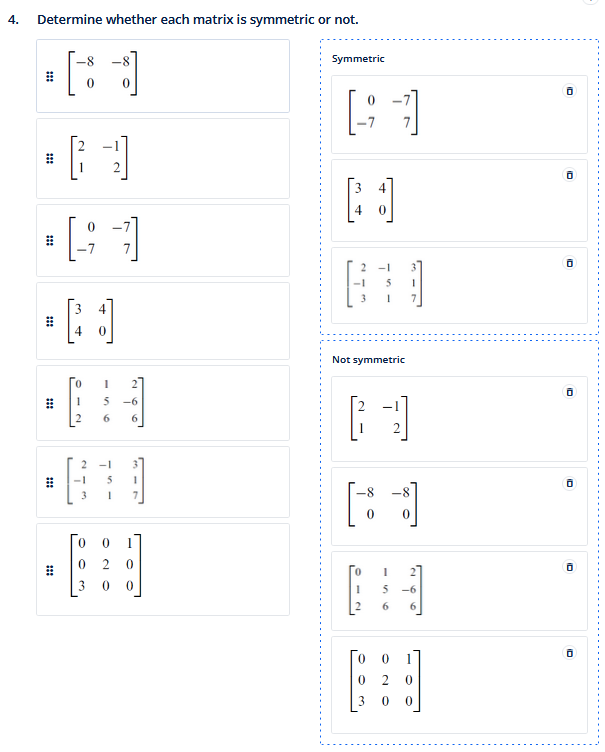
\includegraphics{img/symmetric-or-not.png}

\newpage{}

\hypertarget{find-a-diagonal-matrix-a-that-satisfies-the-given-condition}{%
\paragraph{\texorpdfstring{Find a diagonal matrix \(A\) that satisfies
the given
condition}{Find a diagonal matrix A that satisfies the given condition}}\label{find-a-diagonal-matrix-a-that-satisfies-the-given-condition}}

\begin{enumerate}
\def\labelenumi{\arabic{enumi})}
\tightlist
\item
  \(A^5=\begin{bmatrix}1 & 0 & 0 \\ 0 & -1 & 0 \\ 0 & 0 & -1\end{bmatrix}\)
  \begin{align*}
  A &= \begin{bmatrix}1 & 0 & 0 \\ 0 & -1 & 0 \\ 0 & 0 & -1\end{bmatrix}^{\frac{1}{5}} \\
  &= \begin{bmatrix}1^{\frac{1}{5}} & 0 & 0 \\ 0 & (-1)^{\frac{1}{5}} & 0 \\ 0 & 0 & (-1)^{\frac{1}{5}}\end{bmatrix} \\
  &= \begin{bmatrix}1 & 0 & 0 \\ 0 & -1 & 0 \\ 0 & 0 & -1\end{bmatrix}
  \end{align*}
\item
  \(A^{-2}=\begin{bmatrix}9 & 0 & 0 \\ 0 & 4 & 0 \\ 0 & 0 & 1\end{bmatrix}\)
  \begin{align*}
  A &= \begin{bmatrix}9 & 0 & 0 \\ 0 & 4 & 0 \\ 0 & 0 & 1\end{bmatrix}^{-\frac{1}{2}} \\
  &= \begin{bmatrix}9^{-\frac{1}{2}} & 0 & 0 \\ 0 & 4^{-\frac{1}{2}} & 0 \\ 0 & 0 & 1^{-\frac{1}{2}}\end{bmatrix} \\
  &= \begin{bmatrix}\frac{1}{3} & 0 & 0 \\ 0 & \frac{1}{2} & 0 \\ 0 & 0 & 1\end{bmatrix}
  \end{align*}
\end{enumerate}

\newpage{}

\hypertarget{determinants-and-triangular-matrices-0829}{%
\subsubsection{Determinants and Triangular Matrices
(08/29)}\label{determinants-and-triangular-matrices-0829}}

\hypertarget{what-is-c_32}{%
\paragraph{\texorpdfstring{What is
\(C_{32}\)}{What is C\_\{32\}}}\label{what-is-c_32}}

\(A = \begin{bmatrix}2 & 3 & -1 & 1 \\ -3 & 2 & 0 & 3 \\ 3 & -2 & 1 & 0 \\ 3 & -2 & 1 & 4 \end{bmatrix}\)
\begin{align*}
C_{32} &= (-1)^{3+2}\begin{vmatrix}2 & -1 & 1 \\ -3 & 0 & 3 \\ 3 & 1 & 0\end{vmatrix} \\
&= -\begin{vmatrix}2 & -1 & 1 \\ -3 & 0 & 3 \\ 3 & 1 & 0\end{vmatrix} \\
&= -\left(2\begin{vmatrix}0 & 3 \\ 1 & 0\end{vmatrix}-(-1)\begin{vmatrix}-3 & 3 \\ 3 & 0\end{vmatrix}+1\begin{vmatrix}-3 & 0 \\ 3 & 1\end{vmatrix}\right) \\
&= -\left(2(-3)-(-1)(-9)+1(-3)\right) \\
&= -(-6+9-3) \\
&= 0
\end{align*}

\hypertarget{find-all-values-of-lambda-such-that-a-0}{%
\paragraph{\texorpdfstring{Find all values of \(\lambda\) such that
\textbar{}\(A\)\textbar{} =
0}{Find all values of \textbackslash lambda such that \textbar A\textbar{} = 0}}\label{find-all-values-of-lambda-such-that-a-0}}

\(A = \begin{bmatrix}\lambda-2 & 1 \\ -5 & \lambda+4\end{bmatrix}\)
\begin{align*}
\det(A) &= (\lambda-2)(\lambda+4)-(-5)(1) \\
&= \lambda^2+2\lambda-8+5 \\
&= \lambda^2+2\lambda-3 \\
&= (\lambda+3)(\lambda-1) \\
&= 0
\end{align*}

Therefore, \(\lambda = -3, 1\)

\newpage{}

\hypertarget{for-the-matrix-beginbmatrix3-0-0-2--1-5-1-9--4endbmatrix-find-the-determinant-3-different-ways-with-cofactor-expansion.-pick-different-rows-and-columns-each-time.}{%
\paragraph{\texorpdfstring{For the matrix
\(\begin{bmatrix}3 & 0 & 0 \\2 & -1 & 5 \\ 1 & 9 & -4\end{bmatrix}\)
find the determinant 3 different ways with cofactor expansion. Pick
different rows and columns each
time.}{For the matrix \textbackslash begin\{bmatrix\}3 \& 0 \& 0 \textbackslash\textbackslash2 \& -1 \& 5 \textbackslash\textbackslash{} 1 \& 9 \& -4\textbackslash end\{bmatrix\} find the determinant 3 different ways with cofactor expansion. Pick different rows and columns each time.}}\label{for-the-matrix-beginbmatrix3-0-0-2--1-5-1-9--4endbmatrix-find-the-determinant-3-different-ways-with-cofactor-expansion.-pick-different-rows-and-columns-each-time.}}

\begin{align*}
\det(A) &= 3\begin{vmatrix}-1 & 5 \\ 9 & -4\end{vmatrix}-0\begin{vmatrix}2 & 5 \\ 1 & -4\end{vmatrix}+0\begin{vmatrix}2 & -1 \\ 1 & 9\end{vmatrix} \\
&= 3(-1(-4)-5(9))-0(2(-4)-5(1))+0(2(9)-(-1)(1)) \\
&= 3(4-45)-0(-8-5)+0(18+1) \\
&= 3(-41)-0(-13)+0(19) \\
&= 36
\end{align*}

\begin{align*}
\det(A) &= 0\begin{vmatrix}2 & 5 \\ 9 & -4\end{vmatrix}-3\begin{vmatrix}3 & 0 \\ 1 & -4\end{vmatrix}+0\begin{vmatrix}3 & 0 \\ 2 & 5\end{vmatrix} \\
&= 0(2(-4)-5(9))-3(3(-4)-0(1))+0(3(5)-0(2)) \\
&= 0(-8-45)-3(-12-0)+0(15-0) \\
&= 0(-53)-3(-12) \\
&= 36
\end{align*}

\begin{align*}
\det(A) &= 0\begin{vmatrix}2 & -1 \\ 9 & -4\end{vmatrix}-0\begin{vmatrix}3 & 0 \\ 1 & -4\end{vmatrix}+3\begin{vmatrix}3 & 0 \\ 2 & -1\end{vmatrix} \\
&= 0(2(-4)-(-1)(9))-0(3(-4)-0(1))+3(3(-1)-0(2)) \\
&= 0(-8+9)-0(-12-0)+3(-3-0) \\
&= 0(1)-0(-12)+3(-3) \\
&= 0+0-9 \\
&= 36
\end{align*}

\newpage{}

\hypertarget{evaluate-deta-by-a-cofactor-expansion-along-a-row-or-column-of-your-choice}{%
\paragraph{\texorpdfstring{Evaluate \(\det(A)\) by a cofactor expansion
along a row or column of your
choice}{Evaluate \textbackslash det(A) by a cofactor expansion along a row or column of your choice}}\label{evaluate-deta-by-a-cofactor-expansion-along-a-row-or-column-of-your-choice}}

\(A = \begin{bmatrix}1 & k & k^2 \\ 1 & k & k^2 \\ 1 & k & k^2\end{bmatrix}\)
\begin{align*}
\det(A) &= 1\begin{vmatrix}k & k^2 \\ k & k^2\end{vmatrix}-k\begin{vmatrix}1 & k^2 \\ 1 & k^2\end{vmatrix}+k^2\begin{vmatrix}1 & k \\ 1 & k\end{vmatrix} \\
&= 1(k^2-k^2)-k(1(k^2)-k^2(1))+k^2(1(k)-k(1)) \\
&= 0
\end{align*}

\hypertarget{evaluate-the-determinant-of-the-following-matrices-by-just-looking-at-them.}{%
\paragraph{Evaluate the determinant of the following matrices by just
looking at
them.}\label{evaluate-the-determinant-of-the-following-matrices-by-just-looking-at-them.}}

\(A=\begin{bmatrix}1 & 0 & 0 \\ 0 & -1 & 0 \\ 0 & 0 & 1 \end{bmatrix}\)
\begin{align*}
\det(A) &= 1(-1)(1) = -1
\end{align*}
\(A=\begin{bmatrix}1 & 2 & 7 & -3 \\ 0 & 1 & -4 & 1 \\ 0 & 0 & 2 & 7 \\ 0 & 0 & 0 & 3 \end{bmatrix}\)
\begin{align*}
\det(A) &= 1(1)(2)(3) = 6
\end{align*}

\hypertarget{show-that-the-value-of-the-determinant-is-independent-of-theta}{%
\paragraph{\texorpdfstring{Show that the value of the determinant is
independent of
\(\theta\)}{Show that the value of the determinant is independent of \textbackslash theta}}\label{show-that-the-value-of-the-determinant-is-independent-of-theta}}

\(A=\begin{vmatrix}\sin\theta & \cos\theta & 0 \\ -\cos\theta & \sin\theta & 0 \\ \sin\theta-\cos\theta & \sin\theta+\cos\theta & 1\end{vmatrix}\)
\begin{align*}
\det(A) &= \sin\theta\begin{vmatrix}\sin\theta & 0 \\ \sin\theta+\cos\theta & 1\end{vmatrix}-\cos\theta\begin{vmatrix}\cos\theta & 0 \\ \sin\theta+\cos\theta & 1\end{vmatrix}\\ 
+0\begin{vmatrix}\cos\theta & \sin\theta \\ \sin\theta+\cos\theta & \sin\theta\end{vmatrix} \\
&= \sin\theta\left(\sin\theta(1)-0(\sin\theta+\cos\theta)\right)-\cos\theta\left(\cos\theta(1)-0(\sin\theta+\cos\theta)\right) \\
+0\left(\cos\theta(\sin\theta)-\sin\theta(\sin\theta+\cos\theta)\right) \\
&= \sin^2\theta-\cos^2\theta \\
&= 1
\end{align*}

\newpage{}

\hypertarget{row-operations-and-determinants-0831}{%
\subsubsection{Row operations and Determinants
(08/31)}\label{row-operations-and-determinants-0831}}

\hypertarget{find-the-determinant-of-beginbmatrix1--3-0--2-4-1-5--2-2-endbmatrix-without-using-cofactor-expansion}{%
\paragraph{\texorpdfstring{Find the determinant of
\(\begin{bmatrix}1 & -3 & 0 \\ -2 & 4 & 1 \\ 5 & -2 & 2 \end{bmatrix}\)
WITHOUT using cofactor
expansion}{Find the determinant of \textbackslash begin\{bmatrix\}1 \& -3 \& 0 \textbackslash\textbackslash{} -2 \& 4 \& 1 \textbackslash\textbackslash{} 5 \& -2 \& 2 \textbackslash end\{bmatrix\} WITHOUT using cofactor expansion}}\label{find-the-determinant-of-beginbmatrix1--3-0--2-4-1-5--2-2-endbmatrix-without-using-cofactor-expansion}}

\begin{align*}
\det(A) &= \begin{vmatrix}1 & -3 & 0 \\ -2 & 4 & 1 \\ 5 & -2 & 2 \end{vmatrix} \\
&= \begin{vmatrix}1 & -3 & 0 \\ 0 & -2 & 1 \\ 0 & 13 & 2 \end{vmatrix} \\
&= \begin{vmatrix}1 & -3 & 0 \\ 0 & -2 & 1 \\ 0 & 0 & \frac{28}{2} \end{vmatrix} \\
&= 1(-2)\left(\frac{28}{2}\right) \\
&= -28
\end{align*}

\newpage{}

\hypertarget{find-the-determinant-of-beginbmatrix-2-1-3-1-1-0-1-1-0-2-1-0-0-1-2-3endbmatrix}{%
\paragraph{\texorpdfstring{Find the determinant of
\(\begin{bmatrix} 2 & 1 & 3 & 1 \\ 1 & 0 & 1 & 1 \\ 0 & 2 & 1 & 0 \\ 0 & 1 & 2 & 3\end{bmatrix}\)}{Find the determinant of \textbackslash begin\{bmatrix\} 2 \& 1 \& 3 \& 1 \textbackslash\textbackslash{} 1 \& 0 \& 1 \& 1 \textbackslash\textbackslash{} 0 \& 2 \& 1 \& 0 \textbackslash\textbackslash{} 0 \& 1 \& 2 \& 3\textbackslash end\{bmatrix\}}}\label{find-the-determinant-of-beginbmatrix-2-1-3-1-1-0-1-1-0-2-1-0-0-1-2-3endbmatrix}}

\begin{align*}
\det(A) &= \begin{vmatrix} 2 & 1 & 3 & 1 \\ 1 & 0 & 1 & 1 \\ 0 & 2 & 1 & 0 \\ 0 & 1 & 2 & 3\end{vmatrix} \\
&= \begin{vmatrix} 2 & 1 & 3 & 1 \\ 0 & -2 & -5 & -1 \\ 0 & 2 & 1 & 0 \\ 0 & 1 & 2 & 3\end{vmatrix} \\
&= \begin{vmatrix} 2 & 1 & 3 & 1 \\ 0 & -2 & -5 & -1 \\ 0 & 0 & -4 & -1 \\ 0 & 0 & -3 & 2\end{vmatrix} \\
&= 2(-2)(-4)(2) \\
&= 64
\end{align*}

\newpage{}

\hypertarget{adjoints-and-cramers-rule-0905}{%
\subsubsection{Adjoints and Cramer's Rule
(09/05)}\label{adjoints-and-cramers-rule-0905}}

\hypertarget{find-the-inverse-of-abeginbmatrix2-5-5--1--1-0-2-4-3endbmatrix-using-the-adjoint-method}{%
\paragraph{\texorpdfstring{Find the inverse of
\(A=\begin{bmatrix}2 & 5 & 5 \\ -1 & -1 & 0 \\ 2 & 4 & 3\end{bmatrix}\)
using the adjoint
method}{Find the inverse of A=\textbackslash begin\{bmatrix\}2 \& 5 \& 5 \textbackslash\textbackslash{} -1 \& -1 \& 0 \textbackslash\textbackslash{} 2 \& 4 \& 3\textbackslash end\{bmatrix\} using the adjoint method}}\label{find-the-inverse-of-abeginbmatrix2-5-5--1--1-0-2-4-3endbmatrix-using-the-adjoint-method}}

\begin{align*}
\det(A) &= 2\begin{vmatrix}-1 & 0 \\ 4 & 3\end{vmatrix}-5\begin{vmatrix}-1 & 0 \\ 2 & 3\end{vmatrix}+5\begin{vmatrix}-1 & -1 \\ 2 & 4\end{vmatrix} \\
&= 2(-3)-5(-3)+5(-2) \\
&= -6+15-10 \\
&= -1 \\
\text{adj}(A) &= \begin{bmatrix}(-1)^{1+1}\begin{vmatrix}-1 & 0 \\ 4 & 3\end{vmatrix} & (-1)^{1+2}\begin{vmatrix}-1 & 0 \\ 2 & 3\end{vmatrix} & (-1)^{1+3}\begin{vmatrix}-1 & -1 \\ 2 & 4\end{vmatrix} \\ (-1)^{2+1}\begin{vmatrix}5 & 5 \\ 4 & 3\end{vmatrix} & (-1)^{2+2}\begin{vmatrix}2 & 5 \\ 2 & 3\end{vmatrix} & (-1)^{2+3}\begin{vmatrix}2 & 5 \\ 2 & 4\end{vmatrix} \\ (-1)^{3+1}\begin{vmatrix}5 & 5 \\ -1 & 0\end{vmatrix} & (-1)^{3+2}\begin{vmatrix}2 & 5 \\ -1 & 0\end{vmatrix} & (-1)^{3+3}\begin{vmatrix}2 & 5 \\ -1 & -1\end{vmatrix}\end{bmatrix} \\
&= \begin{bmatrix}(-1)(3) & -(-1)(3) & -4+2 \\ -(15-20) & 6-10 & -(8-10) \\ 5 & -5 & -2+5\end{bmatrix}^T \\
&= \begin{bmatrix}-3 & 3 & -2 \\ 5 & -4 & 2 \\ 5 & -5 & 3\end{bmatrix}^T \\
&= \begin{bmatrix}-3 & 5 & 5 \\ 3 & -4 & -5 \\ -2 & 2 & 3\end{bmatrix} \\
\therefore \ A^{-1} &= -\begin{bmatrix}-3 & 5 & 5 \\ 3 & -4 & -5 \\ -2 & 2 & 3\end{bmatrix} \\
&= \begin{bmatrix}3 & -5 & -5 \\ -3 & 4 & 5 \\ 2 & -2 & -3\end{bmatrix}
\end{align*}

\newpage{}

\hypertarget{solve-the-following-system-of-equations-using-cramers-rule}{%
\paragraph{Solve the following system of equations using Cramer's
Rule}\label{solve-the-following-system-of-equations-using-cramers-rule}}

\systeme{4x+5y=2,11x+y+2z=3,x+5y+2z=1}
\(\longrightarrow \begin{vmatrix} 4 & 5 & 0 \\ 11 & 1 & 2 \\ 1 & 5 & 2\end{vmatrix} \longrightarrow 4\begin{vmatrix}1 & 2 \\ 5 & 2\end{vmatrix}-5\begin{vmatrix}11 & 2 \\ 1 & 2\end{vmatrix} = -132\)
\begin{align*}
\det{(x)} &= \begin{vmatrix}2 & 5 & 0 \\ 3 & 1 & 2 \\ 1 & 5 & 2\end{vmatrix} \\
&= 2\begin{vmatrix}1 & 2 \\ 5 & 2\end{vmatrix}-5\begin{vmatrix}3 & 2 \\ 1 & 2\end{vmatrix} \\
&= 2(2-10)-5(6-2) \\
&= -16-20 \\
&= -36 \\
\det{(y)} &= \begin{vmatrix}4 & 2 & 0 \\ 11 & 3 & 2 \\ 1 & 1 & 2\end{vmatrix} \\
&= 4\begin{vmatrix}3 & 2 \\ 1 & 2\end{vmatrix}-2\begin{vmatrix}11 & 2 \\ 1 & 2\end{vmatrix} \\
&= 4(6-2)-2(22-2) \\
&= 16-40 \\
&= -24 \\
\det{(z)} &= \begin{vmatrix}4 & 5 & 2 \\ 11 & 1 & 3 \\ 1 & 5 & 1\end{vmatrix} \\
&= 4\begin{vmatrix}1 & 3 \\ 5 & 1\end{vmatrix}-5\begin{vmatrix}11 & 3 \\ 1 & 3\end{vmatrix}+2\begin{vmatrix}11 & 1 \\ 1 & 5\end{vmatrix} \\
&= 4(1-15)-5(33-3)+2(55-1) \\
&= -56-150+108 \\
&= -98 \\
\end{align*}

Therefore, the solution
\((x, y, z) = (\frac{3}{11}, \frac{2}{11}, -\frac{49}{66})\)

\newpage{}

\hypertarget{chapter-5-eigenvectors-and-eigenvalues}{%
\section{Chapter 5: Eigenvectors and
Eigenvalues}\label{chapter-5-eigenvectors-and-eigenvalues}}

\hypertarget{eigenvalues-and-eigenvectors-1106}{%
\subsection{Eigenvalues and Eigenvectors
(11/06)}\label{eigenvalues-and-eigenvectors-1106}}

If \(A\) is an \(n \times n\) matrix, then a non-zero vector
\(\symbf{x}\), in \(R^n\), is called an \ul{eigenvector} of \(A\) if
\(A\symbf{x}\) is a scalar multiple of \(\symbf{x}\); that is
\(A\symbf{x} = \lambda\symbf{x}\) for some scalar \(\lambda\). This
scalar \(\lambda\) is called an \ul{eigenvalue} of \(A\) and
\(\symbf{x}\) is said to be an \ul{eigenvector corresponding to}
\(\lambda\).

See, normally, multiplying a vector by a square matrix changes both the
magnitude and the direction of the vector. Really screws it up.

Some examples:

\(\begin{bmatrix}1 & 0 \\ 0 & 1\end{bmatrix}\begin{bmatrix}1 \\ 2\end{bmatrix}=\begin{bmatrix}1 \\ 2\end{bmatrix}\)

\(\begin{bmatrix}1 & 0 \\ 0 & 2 \end{bmatrix}\begin{bmatrix} 1 \\ 2 \end{bmatrix} = \begin{bmatrix}1 \\ 4\end{bmatrix}\)

\(\begin{bmatrix} 5 & 0 \\ 0 & 2 \end{bmatrix}\begin{bmatrix} 1 \\ 2 \end{bmatrix} = \begin{bmatrix} 5 \\ 4 \end{bmatrix}\)

\(\begin{bmatrix}0 & 1 \\ 1 & 0 \end{bmatrix}\begin{bmatrix}1 \\ 2 \end{bmatrix} = \begin{bmatrix}2 \\ 1 \end{bmatrix}\)

\(\begin{bmatrix}1 & 0 \\ 0 & 2\end{bmatrix}\begin{bmatrix}1 \\ 2\end{bmatrix} = \begin{bmatrix}1 \\ 4\end{bmatrix}\)

\(\begin{bmatrix}7 & 8 \\ -2 & 3 \end{bmatrix}\begin{bmatrix}1 \\ 2\end{bmatrix} = \begin{bmatrix}23 \\ 4\end{bmatrix}\)

However, there are some ways to get consistent results.

\hypertarget{examples-2}{%
\subsubsection{Examples}\label{examples-2}}

\hypertarget{vecx-beginbmatrix2-1-endbmatrix-is-an-eigenvector-of-a-beginbmatrix3--2-1-0endbmatrix-because}{%
\paragraph{\texorpdfstring{\(\vec{x} = \begin{bmatrix}2 \\ 1 \end{bmatrix}\)
is an eigenvector of \(A = \begin{bmatrix}3 & -2 \\ 1 & 0\end{bmatrix}\)
because}{\textbackslash vec\{x\} = \textbackslash begin\{bmatrix\}2 \textbackslash\textbackslash{} 1 \textbackslash end\{bmatrix\} is an eigenvector of A = \textbackslash begin\{bmatrix\}3 \& -2 \textbackslash\textbackslash{} 1 \& 0\textbackslash end\{bmatrix\} because}}\label{vecx-beginbmatrix2-1-endbmatrix-is-an-eigenvector-of-a-beginbmatrix3--2-1-0endbmatrix-because}}

\(A\vec{x} = \begin{bmatrix}3 & -2 \\ 1 & 0\end{bmatrix}\begin{bmatrix}2 \\ 1\end{bmatrix} = \begin{bmatrix}4 \\ 2\end{bmatrix} = 2\begin{bmatrix}2 \\ 1\end{bmatrix} = 2\vec{x} \therefore \lambda = 2\)

\hypertarget{let-a-beginbmatrix-1-6-5-2endbmatrix-vecu-beginbmatrix-6--5endbmatrix-vecv-beginbmatrix3--2-endbmatrix.-are-vecu-and-vecv-eigenvectors-of-a}{%
\paragraph{\texorpdfstring{Let
\(A = \begin{bmatrix} 1 & 6 \\ 5 & 2\end{bmatrix}, \vec{u} = \begin{bmatrix} 6 \\ -5\end{bmatrix}, \vec{v} = \begin{bmatrix}3 \\ -2 \end{bmatrix}\).
Are \(\vec{u}\) and \(\vec{v}\) eigenvectors of
\(A\)?}{Let A = \textbackslash begin\{bmatrix\} 1 \& 6 \textbackslash\textbackslash{} 5 \& 2\textbackslash end\{bmatrix\}, \textbackslash vec\{u\} = \textbackslash begin\{bmatrix\} 6 \textbackslash\textbackslash{} -5\textbackslash end\{bmatrix\}, \textbackslash vec\{v\} = \textbackslash begin\{bmatrix\}3 \textbackslash\textbackslash{} -2 \textbackslash end\{bmatrix\}. Are \textbackslash vec\{u\} and \textbackslash vec\{v\} eigenvectors of A?}}\label{let-a-beginbmatrix-1-6-5-2endbmatrix-vecu-beginbmatrix-6--5endbmatrix-vecv-beginbmatrix3--2-endbmatrix.-are-vecu-and-vecv-eigenvectors-of-a}}

\(A\vec{u} = \begin{bmatrix} 1 & 6 \\ 5 & 2\end{bmatrix}\begin{bmatrix} 6 \\ -5\end{bmatrix} = \begin{bmatrix} 1(6)+6(-5) \\ 5(6)+2(-5)\end{bmatrix} = \begin{bmatrix} -24 \\ 20\end{bmatrix} = -4\begin{bmatrix}6 \\ -5\end{bmatrix} \therefore \ \lambda = -4\)

\(A\vec{v} = \begin{bmatrix} 1 & 6 \\ 5 & 2\end{bmatrix}\begin{bmatrix} 3 \\ -2\end{bmatrix} = \begin{bmatrix} 1(3)+6(-2) \\ 5(3)+2(-2)\end{bmatrix} = \begin{bmatrix} -9 \\ 11\end{bmatrix} \neq \lambda\vec{v}\)

\hypertarget{eigenvector-homework-problem-1106}{%
\subsection{Eigenvector Homework Problem
(11/06)}\label{eigenvector-homework-problem-1106}}

\textbf{Confirm by multiplication that \(\symbf{x}\) is an eigenvector
of \(\symbf{A}\), and find the corresponding eigenvalue.}

\hypertarget{a-beginbmatrix4-0-1-2-3-2-1-0-4-endbmatrix-symbfx-beginbmatrix1-2-1endbmatrix}{%
\subsubsection{\texorpdfstring{\(A = \begin{bmatrix}4 & 0 & 1 \\ 2 & 3 & 2 \\ 1 & 0 & 4 \end{bmatrix}; \symbf{x} = \begin{bmatrix}1 \\ 2 \\ 1\end{bmatrix}\)}{A = \textbackslash begin\{bmatrix\}4 \& 0 \& 1 \textbackslash\textbackslash{} 2 \& 3 \& 2 \textbackslash\textbackslash{} 1 \& 0 \& 4 \textbackslash end\{bmatrix\}; \textbackslash symbf\{x\} = \textbackslash begin\{bmatrix\}1 \textbackslash\textbackslash{} 2 \textbackslash\textbackslash{} 1\textbackslash end\{bmatrix\}}}\label{a-beginbmatrix4-0-1-2-3-2-1-0-4-endbmatrix-symbfx-beginbmatrix1-2-1endbmatrix}}

\(A\symbf{x} = \begin{bmatrix}4 & 0 & 1 \\ 2 & 3 & 2 \\ 1 & 0 & 4 \end{bmatrix}\begin{bmatrix}1 \\ 2 \\ 1\end{bmatrix} = \begin{bmatrix}4(1)+0(2)+1(1) \\ 2(1)+3(2)+2(1) \\ 1(1)+0(2)+4(1)\end{bmatrix} = \begin{bmatrix}5 \\ 10 \\ 5\end{bmatrix} = 5\begin{bmatrix}1 \\ 2 \\ 1\end{bmatrix} \therefore \ \lambda = 5\)

\hypertarget{finding-eigenvalues-and-eigenvectors-1107}{%
\subsection{Finding Eigenvalues and Eigenvectors
(11/07)}\label{finding-eigenvalues-and-eigenvectors-1107}}

Essential question:

\textbf{If we know an \(\symbf{n \times n}\) matrix \(\symbf{A}\), can
we find its \(\symbf{\lambda}\)?}

If \(A\vec{x} = \lambda\vec{x}\), then: \begin{align*}
A\vec{x} &= \lambda\vec{x} \\
A\vec{x} - \lambda\vec{x} &= \vec{0} \\
(A-\lambda I)\vec{x} &= \vec{0}
\end{align*} This equation is familiar. It's the homogeneous system of
equations \(A\vec{x} = \vec{0}\), the solution of which is the nullspace
of \(A-\lambda I\). Therefore, \(\vec{x}\) is an eigenvector of
\(A \iff \vec{x}\) is in the nullspace of \(A-\lambda I\).

In this situation, what do we know about that matrix?

Everything in the equivalent statements is false because \(\vec{x}\)
cannot be the zero vector. Therefore, we can see that
\(\det(A-\lambda I)\) OR \(\det(\lambda I-A)\) MUST be 0.

Big Idea: If \(A\) is an \(n \times n\) matrix, then \(\lambda\) is an
eigenvalue of \(A \iff \det(\lambda I-A) = 0\). This is called the
\ul{characteristic equation} of \(A\).

\hypertarget{find-the-characteristic-equation-and-the-eigenvalues-of-abeginbmatrix3-0-5-frac15--1-0-1-1--2endbmatrix}{%
\subsubsection{\texorpdfstring{Find the characteristic equation and the
eigenvalues of
\(A=\begin{bmatrix}3 & 0 & 5\\ \frac{1}{5} & -1 & 0 \\ 1 & 1 & -2\end{bmatrix}\)}{Find the characteristic equation and the eigenvalues of A=\textbackslash begin\{bmatrix\}3 \& 0 \& 5\textbackslash\textbackslash{} \textbackslash frac\{1\}\{5\} \& -1 \& 0 \textbackslash\textbackslash{} 1 \& 1 \& -2\textbackslash end\{bmatrix\}}}\label{find-the-characteristic-equation-and-the-eigenvalues-of-abeginbmatrix3-0-5-frac15--1-0-1-1--2endbmatrix}}

\begin{align*}
\det(\lambda I - A) &= 0 \\
\begin{vmatrix}\lambda-3 & 0 & 5 \\ -\frac{1}{5} & \lambda+1 & 0 \\ -1 & -1 & \lambda+2 \end{vmatrix} &= 0 \\
0 &= (\lambda-3)((\lambda+1)(\lambda+2))+5(\frac{1}{5} + \lambda+1) \\
0 &= (\lambda-3)(\lambda^2+3\lambda+2) \\
0 &= \lambda^3-2\lambda \\
0 &= \lambda(\lambda^2-2)
\lambda &= 0, \pm\sqrt{2}
\end{align*}

\hypertarget{find-the-characteristic-equation-and-the-eigenvalues-of-a-beginbmatrix-1-0-1--1-3-0--4-13--1-endbmatrix}{%
\subsubsection{\texorpdfstring{Find the characteristic equation and the
eigenvalues of
\(A = \begin{bmatrix}-1 & 0 & 1 \\ -1 & 3 & 0 \\ -4 & 13 & -1 \end{bmatrix}\)}{Find the characteristic equation and the eigenvalues of A = \textbackslash begin\{bmatrix\}-1 \& 0 \& 1 \textbackslash\textbackslash{} -1 \& 3 \& 0 \textbackslash\textbackslash{} -4 \& 13 \& -1 \textbackslash end\{bmatrix\}}}\label{find-the-characteristic-equation-and-the-eigenvalues-of-a-beginbmatrix-1-0-1--1-3-0--4-13--1-endbmatrix}}

\begin{align*}
\begin{vmatrix}-1-\lambda & 0 & 1 \\ -1 & 3-\lambda & 0 \\ -4 & 13 & -\lambda \end{vmatrix} = 0 \\
(-1-\lambda) \left((3-\lambda)(-\lambda)-0(13)\right)+\left(-1(13)-(3-\lambda)(-4)\right) &= 0 \\
(-1-\lambda)(\lambda^2-3\lambda)+(-13-4\lambda+12) &= 0 \\
(-1-\lambda)(\lambda^2-3\lambda)+(-4\lambda-1) &= 0 \\
-\lambda^3+3\lambda^2+2 &= 0 \\
(-\lambda+2)(-\lambda^2-\lambda-1) &= 0 \\
(-\lambda+2)(-\lambda-1)(-\lambda+1) &= 0 \\
\lambda &= 2
\end{align*}

\newpage{}

\hypertarget{find-the-eigenvalues-of-a-beginbmatrix2-0-0-6-3-0-1-4-5-endbmatrix}{%
\subsubsection{\texorpdfstring{Find the eigenvalues of
\(A = \begin{bmatrix}2 & 0 & 0 \\ 6 & 3 & 0 \\ 1 & 4 & 5 \end{bmatrix}\)}{Find the eigenvalues of A = \textbackslash begin\{bmatrix\}2 \& 0 \& 0 \textbackslash\textbackslash{} 6 \& 3 \& 0 \textbackslash\textbackslash{} 1 \& 4 \& 5 \textbackslash end\{bmatrix\}}}\label{find-the-eigenvalues-of-a-beginbmatrix2-0-0-6-3-0-1-4-5-endbmatrix}}

\begin{align*}
\begin{vmatrix}\lambda-2 & 0 & 0 \\ 6 & \lambda-3 & 0 \\ 1 & 4 & \lambda-5\end{vmatrix} &= 0 \\
(\lambda-2)(\lambda-3)(\lambda-5) &= 0 \\
\lambda &= 2, 3, 5
\end{align*} Theorem 1: For a triangular matrix, the eigenvalues are the
elements on the main diagonal.

\hypertarget{find-the-eigenvalues-of-a3-if-abeginbmatrixfrac12-4-5--2-0--1-3--8-0-0-2-6-0-0-0-4endbmatrix}{%
\subsubsection{\texorpdfstring{Find the eigenvalues of \(A^3\) if
\(A=\begin{bmatrix}\frac{1}{2} & 4 & 5 & -2 \\ 0 & -1 & 3 & -8 \\ 0 & 0 & 2 & 6 \\ 0 & 0 & 0 & 4\end{bmatrix}\)}{Find the eigenvalues of A\^{}3 if A=\textbackslash begin\{bmatrix\}\textbackslash frac\{1\}\{2\} \& 4 \& 5 \& -2 \textbackslash\textbackslash{} 0 \& -1 \& 3 \& -8 \textbackslash\textbackslash{} 0 \& 0 \& 2 \& 6 \textbackslash\textbackslash{} 0 \& 0 \& 0 \& 4\textbackslash end\{bmatrix\}}}\label{find-the-eigenvalues-of-a3-if-abeginbmatrixfrac12-4-5--2-0--1-3--8-0-0-2-6-0-0-0-4endbmatrix}}

\begin{align*}
\lambda_A = \frac{1}{2}, -1, 2, 4 \\
\lambda_{A^3} = \frac{1}{8}, -1, 8, 64
\end{align*} Theorem 2: The eigenvalues of \(A^k\) are
\(\lambda_1^k, \lambda_2^k, ...\)

\hypertarget{give-me-a-matrix-with-eigenvalues-lambda-0-2-5}{%
\subsubsection{\texorpdfstring{Give me a matrix with eigenvalues
\(\lambda = 0, 2, 5\)}{Give me a matrix with eigenvalues \textbackslash lambda = 0, 2, 5}}\label{give-me-a-matrix-with-eigenvalues-lambda-0-2-5}}

\(A = \begin{bmatrix}0 & 0 & 0 \\ 1 & 2 & 0 \\ 2 & 2 & 5\end{bmatrix}\)

Theorem 3: A square matrix \(A\) is invertible \(\iff \lambda \neq 0\)
(which also means its determinant is 0).

\hypertarget{finding-eigenvectors}{%
\subsubsection{Finding eigenvectors!}\label{finding-eigenvectors}}

Find the nontrivial eigenvectors of:

\(A = \begin{bmatrix}1 & 6 \\ 5 & 2\end{bmatrix}\) \begin{align*}
\begin{vmatrix}\lambda-1 & -6 \\ -5 & \lambda-2\end{vmatrix} &= 0 \\
(\lambda-1)(\lambda-2)-(-6)(-5) &= 0 \\
\lambda^2-3\lambda-28=0 \\
(\lambda-7)(\lambda+4) &= 0 \\
\lambda &= 7, -4
\end{align*} Substitute each \(\lambda\), one at a time into the
\(\lambda I - A\) matrix and find the null space.

For \(\lambda=-4\): \begin{align*}
\left(\begin{array}{cc|c}-5 & -6 & 0 \\ -5 & -6 & 0\end{array}\right) \\
\left(\begin{array}{cc|c}-5 & -6 & 0 \\ 0 & 0 & 0\end{array}\right) \\
\langle-\frac{6}{5}t, t\rangle \\
\vec{x} = \left\{\langle-6, 5\rangle\right\}
\end{align*} For \(\lambda=7\): \begin{align*}
\left(\begin{array}{cc|c}6 & -6 & 0 \\ -5 & 5 & 0\end{array}\right) \\
\left(\begin{array}{cc|c}6 & -6 & 0 \\ 0 & 0 & 0\end{array}\right) \\
\langle t, t\rangle \\
\vec{x} = \left\{\langle6, 6\rangle\right\}
\end{align*} Therefore, the eigen space is:
\(\left\{\langle-6, 5\rangle, \langle6, 6\rangle\right\}\)

\hypertarget{diagonalization-and-similar-triangles}{%
\subsection{Diagonalization and Similar
Triangles}\label{diagonalization-and-similar-triangles}}

Similar matrices: If \(A\) and \(D\) are square matrices, we say that A
and D are ``similar'' if there exists an invertible matrix \(P\) such
that:

\(D = P^{-1}AP\).

\hypertarget{properties-of-similar-matricces}{%
\subsubsection{Properties of Similar
Matricces}\label{properties-of-similar-matricces}}

\begin{itemize}
\tightlist
\item
  They have the same determinant
\item
  If one is invertible, so is the other
\item
  They have the same trace
\item
  They have the same characteristic polynomial
\item
  They have the same eigenvalues
\end{itemize}

\hypertarget{procedure}{%
\subsubsection{Procedure}\label{procedure}}

\begin{enumerate}
\def\labelenumi{\arabic{enumi}.}
\tightlist
\item
  Find the eigenvectors for the \(n \times n\) matrix \(A\).
\end{enumerate}

\begin{itemize}
\tightlist
\item
  Theorem: If an \(n \times n\) matrix \(A\) has \(n\) distinct
  eigenvalues, then \(A\) is \textbf{for sure} diagonalizable.
\end{itemize}

\begin{enumerate}
\def\labelenumi{\arabic{enumi}.}
\setcounter{enumi}{1}
\tightlist
\item
  Make matrix \(P\) out of the eigenveectors (\(P\) is the matrix that
  diagonalizes \(A\))
\item
  Check your work to find matrix \(D\) if reasonable
\end{enumerate}

\hypertarget{example-find-a-matrix-p-that-diagonalizes-a-and-compute-p-1ap}{%
\subsubsection{\texorpdfstring{Example: Find a matrix \(P\) that
diagonalizes \(A\) and compute
\(P^{-1}AP\)}{Example: Find a matrix P that diagonalizes A and compute P\^{}\{-1\}AP}}\label{example-find-a-matrix-p-that-diagonalizes-a-and-compute-p-1ap}}

\begin{enumerate}
\def\labelenumi{\arabic{enumi}.}
\tightlist
\item
  \(A = \begin{bmatrix}3 & 7 \\ 5 & 5 \end{bmatrix}\)
\end{enumerate}

Find the eigenvalues: \begin{align*}
\begin{bmatrix}\lambda-3 & -7 \\ -5 & \lambda-5\end{bmatrix} &= 0 \\
(\lambda-3)(\lambda-5)-(-7)(-5) &= 0 \\
\lambda^2-5\lambda-3\lambda+15-35 &= 0 \\
\lambda^2-8\lambda-20 &= 0 \\
\lambda = -2, 10 
\end{align*}

Find the eigenvectors: \begin{align*}
\lambda = -2: \left[\begin{array}{cc|c}-5 & -7 & 0 \\ -5 & -7 & 0\end{array}\right] 
\vec{x} = \left\{\langle-7, 5\rangle\right\} \\
\lambda = 10: \left[\begin{array}{cc|c}-7 & -7 & 0 \\ -5 & 5 & 0\end{array}\right]
\vec{x} = \left\{\langle1,     1\rangle\right\}
\end{align*}

\newpage{}

Create the matrix \(P\):

\(P = \begin{bmatrix}-7 & 1 \\ 5 & 1\end{bmatrix}\)

Find matrix \(D\): \begin{align*}
D &= P^{-1}AP \\
&= \begin{bmatrix}7 & 1 \\ 5 & -1\end{bmatrix}^{-1}\begin{bmatrix}3 & 7 \\ 5 & 5\end{bmatrix}\begin{bmatrix}7 & 1 \\ 5 & -1\end{bmatrix} \\
&= \begin{bmatrix}-2 & 0 \\ 0 & 10\end{bmatrix}
\end{align*}

\hypertarget{conclusion}{%
\subsubsection{Conclusion}\label{conclusion}}

\begin{itemize}
\tightlist
\item
  If \(D\) has the same eigenvalues of \(A\) and if \(D\) must be
  diagonal, then \(D\) is \textbf{THE} diagonal matrix with eigenvalues
  of \(A\) on the diagonal.
\end{itemize}

\begin{enumerate}
\def\labelenumi{\arabic{enumi}.}
\setcounter{enumi}{1}
\tightlist
\item
  \(A = \begin{bmatrix}2 & 0 & -2 \\ 0 & 3 & 0 \\ 0 & 0 & 1\end{bmatrix}\)
\end{enumerate}

First, find \(D\): \begin{align*}
D = \begin{bmatrix} 2 & 0 & 0 \\ 0 & 3 & 0 \\ 0 & 0 & 1\end{bmatrix} \\
\end{align*}

Then, find \(P\): \begin{align*}
\lambda = 2: \left[\begin{array}{ccc|c}0 & 0 & 2 & 0 \\ 0 & -1 & 0 & 0 \\ 0 & 0 & 1 & 0\end{array}\right] \vec{x} = \langle1, 0, 0\rangle \\
\lambda = 3: \left[\begin{array}{ccc|c}1 & 0 & 2 & 0 \\ 0 & 0 & 0 & 0 \\ 0 & 0 & 2 & 0\end{array}\right] \vec{x} = \langle0, 1, 0\rangle \\
\lambda = 1: \left[\begin{array}{ccc|c}-1 & 0 & 2 & 0 \\ 0 & -2 & 0 & 0 \\ 0 & 0 & 0 & 0\end{array}\right] \vec{x} = \langle2, 0, 1\rangle \\
P = \begin{bmatrix}1 & 0 & 2 \\ 0 & 1 & 0 \\ 0 & 0 & 1\end{bmatrix}
\end{align*}

\hypertarget{more-on-similar-matrices}{%
\subsection{More on Similar Matrices}\label{more-on-similar-matrices}}

There are a few more properties of similar matrices:

\begin{itemize}
\tightlist
\item
  They have the same rank (non-zero eigenvalues)
\item
  They have the same nullity
\item
  They have the same column space
\item
  They have the same row space
\end{itemize}

\hypertarget{example-3}{%
\subsubsection{Example}\label{example-3}}

**Matrix \(A\) is similar to the following matrix:

\(D = \begin{bmatrix}3 & -1 & 1 & 4 & 5 & 2 \\ 0 & -3 & 5 & -10 & -16 & 1 \\ 0 & 0 & 5 & 7 & -8 & 2 \\ 0 & 0 & 0 & 2 & 2 & 0 \\ 0 & 0 & 0 & 0 & 0 & 0 \\ 0 & 0 & 0 & 0 & 0 & 0\end{bmatrix}\)

Rank of \(A\): 4

Nullity of \(A\): 2

Eigenvalues: 3, -3, 5, 2, 0, 0

Characteristic Polynomial: \begin{align*}
\det(\lambda I - A) = 0 \\
\begin{vmatrix}\lambda-3 & 1 & -1 & -4 & -5 & -2 \\ 0 & \lambda+3 & -5 & 10 & 16 & -1 \\ 0 & 0 & \lambda-5 & -7 & 8 & -2 \\ 0 & 0 & 0 & \lambda-2 & -2 & 0 \\ 0 & 0 & 0 & 0 & \lambda & 0 \\ 0 & 0 & 0 & 0 & 0 & \lambda\end{vmatrix} = 0 \\
(\lambda-3)(\lambda+3)(\lambda-5)(\lambda-2)\lambda^2 = 0
\end{align*}

\newpage{}

\hypertarget{some-review}{%
\subsubsection{Some review}\label{some-review}}

\begin{itemize}
\tightlist
\item
  \ul{Eigenspace} of \(\lambda\): The nullspace of \(\lambda I - A\).
  Each eigenvalue will have its own eigenspace.
\item
  \ul{Algebraic multiplicty}: The number of times a given \(\lambda\)
  appears as a root of the characteristic equation.
\item
  \ul{Geometric multiplicity}: The number of eigenvectors it maps to.
\end{itemize}

\hypertarget{theorem-geometric-and-algebraic-multiplicity}{%
\paragraph{Theorem: Geometric and Algebraic
Multiplicity}\label{theorem-geometric-and-algebraic-multiplicity}}

If \(A\) is a square matrix, then: a. For every eigenvalue of \(A\), the
geometric multiplicity is less than or equal to the algebraic
multiplicity. b. \(A\) is diagonalizable \(\iff\) the geometric
multiplicity of each eigenvalue is equal to the algebraic multiplicity.

\hypertarget{similar-matrices-continued-11132023}{%
\subsection{Similar Matrices Continued
(11/13/2023)}\label{similar-matrices-continued-11132023}}

\hypertarget{warm-up}{%
\subsubsection{Warm-Up}\label{warm-up}}

Can you write a new statement involving eigenvalues to add to the list
of equivalent statements?

\(\lambda = 0\) is not an eigenvalue of \(A\)

\hypertarget{homework-review}{%
\subsubsection{Homework Review}\label{homework-review}}

\(A = \begin{bmatrix} 19 & -9 & -6 \\ 25 & -11 & -9 \\ 17 & -9 & -4 \end{bmatrix}\)
\begin{align*}
\begin{bmatrix}\lambda-19 & 9 & 6 \\ -25 & \lambda+11 & 9 \\ 17 & 9 & \lambda + 4\end{bmatrix}
&= (\lambda-19)((\lambda+11)(\lambda+4)-81) + 25(9\lambda+36-54) - 17(81-6\lambda-66) \\
&= (\lambda-1)^2(\lambda-2)
\end{align*}

\(\lambda=1\) has an algebraic multiplicity of 2 and \(\lambda=2\) has
an algebraic multiplicity of 1.

\hypertarget{suppose-that-a-characteristic-polynomial-of-some-matrix-a-is-found-to-be}{%
\subsubsection{\texorpdfstring{Suppose that a characteristic polynomial
of some matrix \(A\) is found to
be:}{Suppose that a characteristic polynomial of some matrix A is found to be:}}\label{suppose-that-a-characteristic-polynomial-of-some-matrix-a-is-found-to-be}}

\(p(\lambda) = (\lambda-1)(\lambda-3)^2(\lambda=4)^3\)

\begin{enumerate}
\def\labelenumi{\alph{enumi}.}
\tightlist
\item
  What are the dimensions of \(A\)?
\end{enumerate}

\(6\times6\)

\begin{enumerate}
\def\labelenumi{\alph{enumi}.}
\setcounter{enumi}{1}
\tightlist
\item
  What are the algebraic multiplicities of each eigenvalue?
\end{enumerate}

\(\lambda=1: 1, \lambda=3:2, \lambda=4:3\)

\begin{enumerate}
\def\labelenumi{\alph{enumi}.}
\setcounter{enumi}{2}
\tightlist
\item
  What are the possible dimensions of the eigenspace associated with
  each of the eigenvalues?
\end{enumerate}

\(\lambda=1:1, \lambda=3:1 \text{ or } 2, \lambda=4:1 \text{ or } 2 \text{ or } 3\)

\begin{enumerate}
\def\labelenumi{\alph{enumi}.}
\setcounter{enumi}{3}
\tightlist
\item
  If \(\{v_1, v_2\}\) is a linearly independent set of eigenvectors of
  \(A\), all of which correspond to the same eigenvalue of \(A\), what
  can you say about the eigenvalue?
\end{enumerate}

The eigenvalue must be 3 or 4.

\hypertarget{semester-ii}{%
\section{Semester II}\label{semester-ii}}

\hypertarget{introduction-to-multivariable-functions-0104}{%
\subsection{Introduction to Multivariable functions
(01/04)}\label{introduction-to-multivariable-functions-0104}}

\hypertarget{definition-of-a-multivariable-function}{%
\subsubsection{Definition of a Multivariable
Function}\label{definition-of-a-multivariable-function}}

Suppose \(D\) is a set of \(n\)-tuples of real numbers
(\(x_1, x_2, ..., x_n\)). A function \(f\) on \(D\) is a rule that
assigns a real number

\(w = f(x_1, x_2, ..., x_n)\)

to each element in \(D\). The set \(D\) is the function's
\textbf{domain}. The set of \(w\)-values taken on by \(f\) is the
function's \textbf{range}. The symbol \(w\) is the \textbf{dependent
variable} of \(f\), and \(f\) is a function of the \(n\)
\textbf{independent variables} \(x_1\) to \(x_n\). The \(x\)'s are the
function's \textbf{input variables}; \(w\) is the function's
\textbf{output variable}.

\hypertarget{limits-and-continuity-0105}{%
\subsection{Limits and Continuity
(01/05)}\label{limits-and-continuity-0105}}

\hypertarget{level-curve-graph-surface}{%
\subsubsection{Level Curve, Graph,
Surface}\label{level-curve-graph-surface}}

The set of points in the plane where a function \(f(x, y)\) has a
constant value \(k\) is called a \textbf{level curve} of \(f\). The
graph of \(f\) is the set of all points \((x, y, z)\) in space, where
\(z = f(x, y)\). The graph of \(f\) is a surface in space.

\hypertarget{limits-with-multivariable-functions}{%
\subsubsection{Limits With Multivariable
Functions}\label{limits-with-multivariable-functions}}

\emph{Limits}: Let \(f\) be a function of two variables defined on an
open region, except possibly at \$(x\_0, \(y_0\)).

In 2-D:

\(\lim_{x\rightarrow c} f(x)\) exists iff
\(\lim_{x\rightarrow c^-} f(x) = \lim_{x\rightarrow c^+} f(x) = L \in \mathbb{R}\)

In 3-D:

\(\lim_{(x, y) \rightarrow (x_0, y_0)} f(x, y)\) exists iff
\(\lim_{(x, y) \rightarrow (x_0, y_0)^-} f(x, y) = L \in \mathbb{R}\)
from \ul{all} directions.

\hypertarget{examples-3}{%
\subsubsection{Examples}\label{examples-3}}

\begin{enumerate}
\def\labelenumi{\arabic{enumi}.}
\item
  \(\lim_{(x, y) \rightarrow (1, 2)} \cfrac{5x^2y}{x^2+y^2} = \cfrac{5 \cdot 1 \cdot 2}{1 + 4} = \cfrac{10}{5} = 2\)
\item
  \(\lim_{(x, y) \rightarrow (1, 1)} \cfrac{x-y}{x^2-y^2} = \cfrac{0}{0}\)
\end{enumerate}

Since this is indeterminate, you need to switch to traditional limit
solving methods. There is no \emph{L'Hopital's Rule} for multivariable
functions. Instead, factor the numerator and denominator and cancel out
common factors.

\(\lim_{(x, y) \rightarrow (1, 1)} \cfrac{x-y}{(x-y)(x+y)} = \cfrac{1}{2}\)

\begin{enumerate}
\def\labelenumi{\arabic{enumi}.}
\setcounter{enumi}{2}
\tightlist
\item
  \(\lim_{(x, y) \rightarrow (4, 3)} \cfrac{\sqrt{x}-\sqrt{y+1}}{x-y-1}\)
\end{enumerate}

\hypertarget{homework}{%
\subsubsection{Homework}\label{homework}}

\hypertarget{evaluate-the-limit-lim_x-y-rightarrow-0-0-cfrac3x2-y25x2y22}{%
\paragraph{\texorpdfstring{Evaluate the limit
\(\lim_{(x, y) \rightarrow (0, 0)} \cfrac{3x^2-y^2+5}{x^2+y^2+2}\)}{Evaluate the limit \textbackslash lim\_\{(x, y) \textbackslash rightarrow (0, 0)\} \textbackslash cfrac\{3x\^{}2-y\^{}2+5\}\{x\^{}2+y\^{}2+2\}}}\label{evaluate-the-limit-lim_x-y-rightarrow-0-0-cfrac3x2-y25x2y22}}

\(\left.\lim_{(x, y) \rightarrow (0, 0)} \cfrac{3x^2-y^2+5}{x^2+y^2+2}\right\vert_{(0,0)} = \cfrac{5}{2}\)

\hypertarget{evaluate-the-limit-lim_x-y-rightarrow-1-1-cossqrt3xy-1}{%
\paragraph{\texorpdfstring{Evaluate the limit
\(\lim_{(x, y) \rightarrow (1, 1)} \cos\sqrt[3]{|xy|-1}\)}{Evaluate the limit \textbackslash lim\_\{(x, y) \textbackslash rightarrow (1, 1)\} \textbackslash cos\textbackslash sqrt{[}3{]}\{\textbar xy\textbar-1\}}}\label{evaluate-the-limit-lim_x-y-rightarrow-1-1-cossqrt3xy-1}}

\(\left.\lim_{(x, y) \rightarrow (1, 1)} \cos\sqrt[3]{|xy|-1}\right\vert_{(1, 1} = \cos0 = 1\)

\hypertarget{evaluate-the-limit-lim_x-y-rightarrow-1-1-cfracxy-y-2x2x-1}{%
\paragraph{\texorpdfstring{Evaluate the limit
\(\lim_{(x, y) \rightarrow (1, 1)} \cfrac{xy-y-2x+2}{x-1}\)}{Evaluate the limit \textbackslash lim\_\{(x, y) \textbackslash rightarrow (1, 1)\} \textbackslash cfrac\{xy-y-2x+2\}\{x-1\}}}\label{evaluate-the-limit-lim_x-y-rightarrow-1-1-cfracxy-y-2x2x-1}}

\(\lim_{(x, y) \rightarrow (1, 1)} \cfrac{xy-y-2x+2}{x-1}=\cfrac{(x-1)(y-2)}{x-1}=\left.y-2\right\vert_{(1,1)} = -1\)

\hypertarget{on-what-interval-is-the-function-fx-y-sinxy-continuous}{%
\paragraph{\texorpdfstring{On what interval is the function
\(f(x, y) = \sin(x+y)\)
continuous?}{On what interval is the function f(x, y) = \textbackslash sin(x+y) continuous?}}\label{on-what-interval-is-the-function-fx-y-sinxy-continuous}}

The \(\sin\) function is continuous everywhere, so
\((x, y) \in \mathbb{R}^2\)

\hypertarget{on-what-interval-is-the-function-fx-y-z-x2y2-2z2-continuous}{%
\paragraph{\texorpdfstring{On what interval is the function
\(f(x, y, z) = x^2+y^2-2z^2\)
continuous?}{On what interval is the function f(x, y, z) = x\^{}2+y\^{}2-2z\^{}2 continuous?}}\label{on-what-interval-is-the-function-fx-y-z-x2y2-2z2-continuous}}

\((x, y, z) \in \mathbb{R}^3\)

\hypertarget{on-what-interval-is-the-function-fx-y-z-xysinleftfrac1zright-continuous}{%
\paragraph{\texorpdfstring{On what interval is the function
\(f(x, y, z) = xy\sin\left(\frac{1}{z}\right)\)
continuous?}{On what interval is the function f(x, y, z) = xy\textbackslash sin\textbackslash left(\textbackslash frac\{1\}\{z\}\textbackslash right) continuous?}}\label{on-what-interval-is-the-function-fx-y-z-xysinleftfrac1zright-continuous}}

Can't divide by zero, so \((x, y, z) \in \mathbb{R}^3 | z \ne 0\)

\hypertarget{limits-that-do-not-exist-in-3-space-0108}{%
\subsection{Limits that DO NOT EXIST in 3-Space
(01/08)}\label{limits-that-do-not-exist-in-3-space-0108}}

\hypertarget{question-does-the-function-fxy-cfrac2x2yx4y2-have-a-limit-as-xy-approaches-00}{%
\subsubsection{\texorpdfstring{Question: Does the function
\(f(x,y) = \cfrac{2x^2y}{x^4+y^2}\) have a limit as (x,y) approaches
(0,0)?}{Question: Does the function f(x,y) = \textbackslash cfrac\{2x\^{}2y\}\{x\^{}4+y\^{}2\} have a limit as (x,y) approaches (0,0)?}}\label{question-does-the-function-fxy-cfrac2x2yx4y2-have-a-limit-as-xy-approaches-00}}

Nope, it approaches the point differently.

\hypertarget{find-left.fx-yrightvert_yx2-and-compute-lim_x-y-rightarrow-0-0-fx-y-along-yx2}{%
\subsubsection{\texorpdfstring{Find \(\left.f(x, y)\right\vert_{y=x^2}\)
and compute \(\lim_{(x, y) \rightarrow (0, 0)} f(x, y)\) along
\(y=x^2\)}{Find \textbackslash left.f(x, y)\textbackslash right\textbackslash vert\_\{y=x\^{}2\} and compute \textbackslash lim\_\{(x, y) \textbackslash rightarrow (0, 0)\} f(x, y) along y=x\^{}2}}\label{find-left.fx-yrightvert_yx2-and-compute-lim_x-y-rightarrow-0-0-fx-y-along-yx2}}

\(\left.f(x,y) = \cfrac{2x^2y}{x^4 +y^2}\right\vert_{y=x^2} = \cfrac{2x^4}{2x^4} = 1\)

\hypertarget{find-left.fx-yrightvert_y-x2-and-compute-lim_x-y-rightarrow-0-0-fx-y-along-y-x2}{%
\subsubsection{\texorpdfstring{Find
\(\left.f(x, y)\right\vert_{y=-x^2}\) and compute
\(\lim_{(x, y) \rightarrow (0, 0)} f(x, y)\) along
\(y=-x^2\)}{Find \textbackslash left.f(x, y)\textbackslash right\textbackslash vert\_\{y=-x\^{}2\} and compute \textbackslash lim\_\{(x, y) \textbackslash rightarrow (0, 0)\} f(x, y) along y=-x\^{}2}}\label{find-left.fx-yrightvert_y-x2-and-compute-lim_x-y-rightarrow-0-0-fx-y-along-y-x2}}

\(\left.f(x,y) = \cfrac{2x^2y}{x^4 +y^2}\right\vert_{y=x^2} = \cfrac{-2x^4}{2x^4} = 1\)

\hypertarget{explain-why-we-can-conclude-that-lim_x-y-rightarrow-0-0-fxy-does-not-exist}{%
\subsubsection{\texorpdfstring{Explain why we can conclude that
\(\lim_{(x, y) \rightarrow (0, 0)} f(x,y)\) does not
exist}{Explain why we can conclude that \textbackslash lim\_\{(x, y) \textbackslash rightarrow (0, 0)\} f(x,y) does not exist}}\label{explain-why-we-can-conclude-that-lim_x-y-rightarrow-0-0-fxy-does-not-exist}}

\(\lim_{(x,y) \rightarrow(0,0)}f(x,y)\) along \(y=x^2\)
\(\ne \lim_{(x, y)\rightarrow(0, 0)}f(x, y)\) along \(y=-x^2\)

\hypertarget{how-did-we-know-to-choose-yx2-and-y-x2-to-evaluate-the-limit}{%
\subsubsection{\texorpdfstring{How did we know to choose \(y=x^2\) and
\(y=-x^2\) to evaluate the
limit?}{How did we know to choose y=x\^{}2 and y=-x\^{}2 to evaluate the limit?}}\label{how-did-we-know-to-choose-yx2-and-y-x2-to-evaluate-the-limit}}

You want to try to choose things that, as you plug them in, you get a
nice expression that you can simplify. For this prblem in particular, we
chose paths towards \((0, 0)\) that, when substituted, would be easy to
solve and yield different answers upon simplification. We could've also
used the equation of the x-axis (\(y=0\)).

\hypertarget{show-that-these-functions-have-no-limit-as-x-y-approaches-0-0-by-considering-different-paths-of-approach.}{%
\subsubsection{\texorpdfstring{Show that these functions have no limit
as \((x, y)\) approaches \((0, 0)\) by considering different paths of
approach.}{Show that these functions have no limit as (x, y) approaches (0, 0) by considering different paths of approach.}}\label{show-that-these-functions-have-no-limit-as-x-y-approaches-0-0-by-considering-different-paths-of-approach.}}

\hypertarget{fxy-cfracx4x4y2}{%
\paragraph{\texorpdfstring{\(f(x,y) = \cfrac{x^4}{x^4+y^2}\)}{f(x,y) = \textbackslash cfrac\{x\^{}4\}\{x\^{}4+y\^{}2\}}}\label{fxy-cfracx4x4y2}}

\(\lim_{(x, y)\rightarrow(0, 0)} f(x, y)\) along
\(y=2x^2 = \cfrac{x^4}{5x^4}=\cfrac{1}{5}\)
\(\ne \lim_{(x, y)\rightarrow(0, 0)} f(x, y)\) along
\(y=x^2 = \cfrac{x^4}{2x^4} = \cfrac{1}{2}\)

\hypertarget{fx-y-cfracx2yy}{%
\paragraph{\texorpdfstring{\(f(x, y) = \cfrac{x^2+y}{y}\)}{f(x, y) = \textbackslash cfrac\{x\^{}2+y\}\{y\}}}\label{fx-y-cfracx2yy}}

\(\lim_{(x, y)\rightarrow(0,0)} f(x, y)\) along
\(y=x^2 = \cfrac{2y}{y} = 2\)
\(\ne \lim_{(x, y)\rightarrow(0,0)} f(x, y)\) along
\(y=2x^2 = \cfrac{3x^2}{2x^2} = \cfrac{3}{2}\)



\end{document}
